%======================================================================
%   D O C U M E N T   P R E A M B L E
% Specify the document class, default style attributes, and page dimensions, etc.
% For hyperlinked PDF, suitable for viewing on a computer, use this:
\documentclass[letterpaper,12pt,oneside,final]{article}
 
% For PDF, suitable for double-sided printing, change the PrintVersion variable below to "true" and use this \documentclass line instead of the one above:
%\documentclass[letterpaper,12pt,titlepage,openright,twoside,final]{book}
\newcommand{\package}[1]{\textbf{#1}} % package names in bold text
\newcommand{\cmmd}[1]{\textbackslash\texttt{#1}} % command name in tt font 
\newcommand{\href}[1]{#1} % does nothing, but defines the command so the print-optimized version will ignore \href tags (redefined by hyperref pkg).
%\newcommand{\texorpdfstring}[2]{#1} % does nothing, but defines the command
% Anything defined here may be redefined by packages added below...

%\usepackage{nomencl} % For a nomenclature (optional; available from ctan.org)
\usepackage{amsmath,amssymb,amstext} % Lots of math symbols and environments
\usepackage[pdftex]{graphicx} % For including graphics N.B. pdftex graphics driver
\usepackage{amsmath,amssymb,amstext,amsthm,amsfonts}
\usepackage{dsfont}
\usepackage[pdftex]{graphicx}
\usepackage{caption}
\usepackage{color}% Include colors for document elements
\usepackage{dcolumn}% Align table columns on decimal point
\usepackage{bm}% bold math
\usepackage{float}
\usepackage{multirow}
%\usepackage{natbib}   % omit 'round' option for square brackets

\usepackage{algorithm} % For counting chapters
\usepackage{algorithmicx, algpseudocode}
%\renewcommand{\algorithmiccomment}[1]{// #1} % Brackets are confused with the sets
%\algsetup{linenosize=\scriptsize}

% N.B. HYPERREF MUST BE THE LAST PACKAGE LOADED; ADD ADDITIONAL PKGS ABOVE
\usepackage[pdftex,pagebackref=false]{hyperref} % with basic options
%\usepackage[pdftex,pagebackref=true]{hyperref}
% N.B. pagebackref=true provides links back from the References to the body text. This can cause trouble for printing.
% define colours
\definecolor{background-color}{gray}{0.98}
\definecolor{steelblue}{rgb}{0.27, 0.51, 0.71}
\definecolor{brickred}{rgb}{0.8, 0.25, 0.33}
\definecolor{bluegray}{rgb}{0.4, 0.6, 0.8}
\definecolor{amethyst}{rgb}{0.6, 0.4, 0.8}

\hypersetup{
    plainpages=false,       % needed if Roman numbers in frontpages
    unicode=false,          % non-Latin characters in Acrobat's bookmarks
    pdftoolbar=true,        % show Acrobats toolbar?
    pdfmenubar=true,        % show Acrobat's menu?
    pdffitwindow=false,     % window fit to page when opened
    pdfstartview={FitH},    % fits the width of the page to the window
    pdftitle={Toeplitz\ Eigenvalues},    % title: CHANGE THIS TEXT!
    pdfauthor={Chris Salahub},    % author: CHANGE THIS TEXT! and uncomment this line
    pdfsubject={Statistics},  % subject: CHANGE THIS TEXT! and uncomment this line
%    pdfkeywords={keyword1} {key2} {key3}, % list of keywords, and uncomment this line if desired
    pdfnewwindow=true,      % links in new window
    colorlinks=true,        % false: boxed links; true: colored links
    linkcolor=steelblue,         % color of internal links
    citecolor=brickred,        % color of links to bibliography
    filecolor=magenta,      % color of file links
    urlcolor=cyan           % color of external links
}

% Page margins
% uWaterloo thesis requirements specify a minimum of 1 inch (72pt) margin at the
% top, bottom, and outside page edges and a 1.125 in. (81pt) gutter margin (on binding side). 
\setlength{\marginparwidth}{0pt} % width of margin notes
% N.B. If margin notes are used, you must adjust \textwidth, \marginparwidth
% and \marginparsep so that the space left between the margin notes and page
% edge is less than 15 mm (0.6 in.)
\setlength{\marginparsep}{0pt} % width of space between body text and margin notes
\setlength{\evensidemargin}{0.125in} % Adds 1/8 in. to binding side of all even pages when "twoside" is selected
\setlength{\oddsidemargin}{0.125in} % Adds 1/8 in. to the left of all pages when "oneside" is selected,
                                    % and to the left of all odd pages when "twoside" is selected
\setlength{\textwidth}{6.375in} % assuming US letter paper (8.5 in. x 11 in.) and margins as above
\raggedbottom

\setlength{\parskip}{\medskipamount} % space between paragraphs
\renewcommand{\baselinestretch}{1} % line space setting

% Commands
% Code
\newcommand{\code}[1]{\texttt{#1}}
\newcommand*{\Rnsp}{\textsf{R}}
\newcommand*{\R}{\textsf{R}$~$}
\newcommand*{\Pythonnsp}{\textsf{Python}}
\newcommand*{\Python}{\textsf{Python}$~$}
\newcommand{\pkg}[1]{\textsf{#1}}
\newcommand{\pkgsp}[1]{\textsf{#1}$~$}
\algblock{Input}{EndInput}
\algnotext{EndInput}
\newcommand{\Desc}[2]{\State \makebox[2em][l]{#1}#2}

% Theorem styles
\newtheorem{definition}{Definition}
\newtheorem{theorem}{Theorem}

% vectors
\newcommand{\ve}[1]{\mathbf{#1}}           % for vectors
\newcommand{\sv}[1]{\boldsymbol{#1}}   % for greek letters
\newcommand{\m}[1]{\mathbf{#1}}               % for matrices
\newcommand{\sm}[1]{\boldsymbol{#1}}   % for greek letters
\newcommand{\tr}[1]{{#1}^{\mkern-1.5mu\mathsf{T}}}              % for transpose
\newcommand{\conj}[1]{{#1}^{\ast}}
\newcommand{\norm}[1]{||{#1}||}              % norm
\newcommand{\frob}[1]{\norm{#1}_F}
\newcommand{\abs}[1]{\lvert{#1}\rvert}              % norm
\newcommand*{\mvec}{\operatorname{vec}}
\newcommand*{\trace}{\operatorname{trace}}
\newcommand*{\rank}{\operatorname{rank}}
\newcommand*{\diag}{\operatorname{diag}}
\newcommand*{\vspan}{\operatorname{span}}
\newcommand*{\rowsp}{\operatorname{rowsp}}
\newcommand*{\colsp}{\operatorname{colsp}}
\newcommand*{\svd}{\operatorname{svd}}
\newcommand*{\edm}{\operatorname{edm}}  % euclidean distance matrix (D * D)
\newcommand{\oneblock}[3]{\m{B}_{#1:#2:#3}}
\newcommand{\stripe}[2]{\m{S}_{#1,#2}}

% contingency tables
\newcommand{\abdiff}{\delta_{AB}}

% statistical
\newcommand{\widebar}[1]{\overline{#1}}  
\newcommand{\wig}[1]{\tilde{#1}}  
\newcommand{\bigwig}[1]{\widetilde{#1}}  
\newcommand{\follows}{\sim}  
\newcommand{\leftgiven}{~\left\lvert~}
\newcommand{\given}{~\vert~}
\newcommand{\biggiven}{~\vline~}
\newcommand{\indep}{\bot\hspace{-.6em}\bot}
\newcommand{\notindep}{\bot\hspace{-.6em}\bot\hspace{-0.75em}/\hspace{.4em}}
\newcommand{\depend}{\Join}
\newcommand{\notdepend}{\Join\hspace{-0.9 em}/\hspace{.4em}}
\newcommand{\imply}{\Longrightarrow}
\newcommand{\notimply}{\Longrightarrow \hspace{-1.5em}/ \hspace{0.8em}}
\newcommand{\xyAssociation}{g}
\newcommand{\xDomain}{\mathcal{X}}
\newcommand{\yDomain}{\mathcal{Y}}
\newcommand{\measureRange}{\mathcal{R}}
\newcommand{\bigChi}{\mathcal{D}}
\newcommand{\ind}[2]{I_{#2} \left( #1 \right)}
%\newcommand{\ind}[1]{\mathds{1} \hspace{-0.1cm}\left( #1 \right)}
\newcommand{\mutInf}{\mathcal{I}}
 
% operators
\newcommand{\Had}{\circ}
\newcommand{\measureAssociation}{G}
\DeclareMathOperator*{\lmin}{Minimize}
\DeclareMathOperator*{\argmin}{arg\,min}
\DeclareMathOperator*{\argmax}{arg\,max}
\DeclareMathOperator*{\arginf}{arg\,inf}
\DeclareMathOperator*{\argsup}{arg\,sup}

% Sets
\newcommand*{\intersect}{\cap}
\newcommand*{\union}{\cup}
\let\oldemptyset\emptyset
\let\emptyset\varnothing

% Fields, Reals, etc. etc
\newcommand{\field}[1]{\mathbb{#1}}
\newcommand{\Reals}{\field{R}}
\newcommand{\Integers}{\field{Z}}
\newcommand{\Naturals}{\field{N}}
\newcommand{\Complex}{\field{C}}
\newcommand{\Rationals}{\field{Q}}

% Editorial
\newcommand{\needtocite}[1]{{\color{red} [Need to cite {#1} here]}}
\newcommand{\comment}[1]{{\color{steelblue} COMMENT:  {#1}}}
\newcommand{\TODO}[1]{{\color{brickred} TODO:  {#1}}}

\title{Circulant matrices and eigenvalue-based $p$-value adjustment for multiple testing in genetics.}
\author{Chris Salahub \\ {\footnotesize University of Waterloo, \texttt{csalahub@uwaterloo.ca}}}

\begin{document}

\maketitle

\section{Introduction}

Suppose each of a collection of $M$ independent variables $X_1, \dots, X_M$ is tested against a common dependent variable $Y$ with a pairwise measure $g(X_i, Y)$ in order to screen $X_1, \dots, X_M$ for association with $Y$. Though this practice is not ideal for determining the complete dependency, as a subset of the $X$ with individually low $g$ values may collectively be highly associated with $Y$, when $M$ is particularly large it is common practice.

The combinatorial explosion of all possible subsets of $M$ variables presents a serious computational barrier to such complete modelling, while it is conceptually difficult to think of function which would provide a universal comparison between these subsets. Even if these computational and conceptual burdens are overcome, some repeated measurement of $g$ over thousands of combinations occurs. This introduces an unavoidable multiple testing problem. Values of $g$ which would be significant if observed alone are less meaningful when observed in a collection of thousands of values.

Restricting ourselves to the binary case where we have $\ve{g} = \{g(X_i, Y)\}_{i = 1, \dots, M}$, a number of adjustments for the problem of $M$ repeated tests exist surveyed in literature such as \cite{cousins2008pooling, cinarviechtbauer2022poolr}. The simplest of these is the Bonferroni correction. If the individual significance level is chosen to be $\alpha$, this correction applies the adjustment
$$\frac{\alpha}{M}$$
and uses this significance level to assess each test. This method is known to be overly conservative and does not take any of the structure of $X_1, \dots, X_M$ into account.

A collection of approaches outlined in \cite{cinarviechtbauer2022poolr} attempts to use the correlation structure of $X_1, \dots, X_M$ to relax the Bonferroni correction. The central idea to this relaxation is that strongly dependent tests do not all deserve a weight of one when counting the number of tests for adjustment. Rather, these tests should be combined into an effective count less than the count of variables. Inspired by the use of principal components analysis (PCA) to reduce dimension by selecting the top eigendirections, these methods take
$$M_{\text{eff}} = f(\lambda_1, \lambda_2, \dots, \lambda_M) = f(\sv{\lambda})$$
where $\sv{\lambda}$ are the $M$ eigenvalues of $\sm{\Sigma}$, the correlation matrix of the $X_i$. This collection includes \cite{cheverud2001, nyholt2004, LiJi2005, Galwey2009}.

Besides inspiration, these test adjustments share a common motivation: the identification of genetic factors in traits and disease through genome-wide association studies (GWAS). \cite{uffelmannetal2021gwas} provides a good survey of GWAS practice. The typical GWAS will measure $M$ positions on the genome and compare each of these to a single measurable trait $Y$. These $M$ measured positions will have highly structured correlations between them due to the organization of genetic information in DNA. GWAS are also frequently mentioned in the literature on measures of association, such as \cite{reshef2011MIC, liuetal2018kernel}. This shared motivation therefore deserves special attention. Indeed, much can be shown about the structure of genetic measurements as collected in a GWAS.

\section{Multiple testing}

\subsection{Notation}

Suppose $\bigwig{\sv{\mu}} \follows N_M (\sv{\mu}, \sm{\Sigma})$ where $\sm{\Sigma} = [\rho_{ij}]$ is a correlation matrix so that $\rho_{ii} = 1$, $ \rho_{ij} = \rho_{ji}$, and $\abs{\rho_{ij}} \le 1$ for all $i = 1, \ldots M$ and $j = 1, \ldots M$.

Let $\sm{\Sigma} = \m{V} \m{D}_\lambda \tr{\m{V}}$ be its eigen decomposition with 
$\m{D}_\lambda = diagonal(\lambda_1, \lambda_2, \ldots, \lambda_M)$ 
the diagonal matrix of eigenvalues $\lambda_1 \ge \lambda_2 \ge \cdots \lambda_M \ge 0$
and $M \times M$ orthogonal matrix
$\m{V} = [\ve{V}_1 | \ve{V}_2 | \cdots | \ve{V}_M]$ having as columns the $M \times 1$ eigenvectors $\ve{V}_i$ corresponding to each eigenvalue $\lambda_i$ for $i = 1, \ldots n$.

Note that for the special case of $\rho_{ij} = \rho > 0$ for all $i \ne j$, $\sm{\Sigma}$ can be written as
\begin{equation}
 \sm{\Sigma} = \rho \ve{1} \tr{\ve{1}} + (1 - \rho) \m{I}_M 
\label{eq:multipleTesting:commonCor}
\end{equation}
where $\ve{1} = \tr{(1, 1, \ldots, 1)}$ is the $M \times 1$ vector of ones and $\m{I}_M$ the $M \times M$ identity matrix.  In this case, $\lambda_ 1 = (M - 1) \rho + 1$ and $\lambda_2 = \lambda_3 = \cdots = \lambda_M = (1 - \rho)$.  The corresponding eigenvectors  are $\ve{V}_1 = \frac{1}{\sqrt{M}} \ve{1}$ and any linearly independent set of $(M - 1)$ orthonormal vectors $\ve{V}_2, \ldots, \ve{V}_M$ all orthogonal to $\ve{V}_1$.  
Note that if $\rho < 0$, the eigen decomposition is the same but $\lambda = (M-1)\rho +1$ would be the \emph{smallest} eigenvalue and $\sm{\Sigma}$ would be a non-negative definite matrix only when $\rho \ge -1/(M-1)$.

Of interest is testing the hypothesis $H_0: \sv{\mu} = \ve{0}$ having observed some realization $\widehat{\sv{\mu}}$ of $\bigwig{\sv{\mu}}$.  Equivalently, the $M$ hypotheses $H_{0i}: \mu_i = 0$ might be tested independently and simultaneously based on the marginal distributions $\bigwig{\mu}_i \follows N(\mu_i, 1)$ and observed $\widehat{\mu}_i$ for $i = 1, \ldots, M$.  The challenge is combining these as a test for $H_0$.

Testing any of these hypotheses for a fixed significance level $\alpha$ is equivalent to forming confidence regions of size $1 - \alpha$ and determining whether the region contains 0 for a univariate test of $H_{0i}$ or the $M \times 1$ vector $\ve{0}$ for the multivariate test of $H_0$.   A fixed level test would reject the hypothesis whenever the corresponding region did not contain the zero value and would accept otherwise.

\subsection{The Multivariate Test}
For the multivariate test the confidence region would be the set of all $\sv{\mu}$  which satisfy
\begin{equation}
\tr{(\sv{\mu} - \widehat{\sv{\mu}})} {\sm{\Sigma}}^{-1} (\sv{\mu} - \widehat{\sv{\mu}}) \le C_\alpha
\label{eq:multipleTesting:mvnconf}
\end{equation}
where $C_\alpha$ is the critical value found from a $\chi^2$ distribution on $M$ degrees of freedom as
\[ Pr(\chi_M^2 \le C_\alpha) = 1 - \alpha. \]
For example, when $\alpha = 0.05$ and $M =  2$,  $C_\alpha \approx 5.99$ and Equation (\ref{eq:multipleTesting:mvnconf}) determines the $95\%$ confidence region for $\sv{\mu}$.

The shape of this confidence region is an $M$-dimensional ellipsoid centred at $\widehat{\sv{\mu}}$. Points outside the ellipse would be rejected by a level $\alpha = 0.05$ test while those inside would be accepted. Testing $H_0: \sv{\mu} = \ve{0}$ is equivalent to checking whether the origin $\ve{0}$ is outside the ellipse or not. %Figure \ref{fig:ellipsesRhos} 
%\begin{figure}[htp]
%\begin{center}
%\begin{tabular}{cccc}
%\includegraphics[width = 0.220\textwidth]{./img/ellipseRho0.png} &
%\includegraphics[width = 0.220\textwidth]{./img/ellipseRho5.png} &
%\includegraphics[width = 0.220\textwidth]{./img/ellipseRho9.png} &
%\includegraphics[width = 0.220\textwidth]{./img/ellipseRho10.png} \\
%{\footnotesize (a) $\rho = 0$} &
%{\footnotesize (b) $\rho = 0.5$} &
%{\footnotesize (c) $\rho = 0.9$} &
%{\footnotesize (d) $\rho = 1$} 
%\end{tabular}
%\end{center}
%\caption{95 \% confidence regions ($\alpha = 0.05$) centred about $\widehat{\sv{\mu}}$ for various values of $\rho$.  These are derived from Equation (\ref{eq:mvnconf}) when $M = 2$.  In all cases, values of $\sv{\mu}^{(i)}$ would be accepted at a fixed significance level of $\alpha = 0.05$ if inside the ellipse and rejected if outside. Grid shows unit squares.}
%\label{fig:ellipsesRhos}
%\end{figure}
%shows the $95\%$ confidence regions for $\sv{\mu}$ when $M = 2$ for various values of the correlation $\rho$.  The region is an ellipse centred at $\widehat{\sv{\mu}}$; it is a perfect circle when $\rho = 0$ and becomes increasingly narrower as $\rho$ increases until it becomes a line segment when $\rho = 1$.  

%Each plot of Figure \ref{fig:ellipsesRhos} also shows three different possible values (viz. $\sv{\mu}^{(1)}$, 
%$\sv{\mu}^{(2)}$, and $\sv{\mu}^{(3)}$) for $\sv{\mu}$.  Those points outside the ellipse would be rejected by a level $\alpha = 0.05$ test; those inside would be accepted. To test $H_0: \sv{\mu} = \ve{0}$ we just see whether the origin $\ve{0}$ is outside the ellipse or not.  If for example, $\sv{\mu}^{(1)} = \ve{0}$ in Figure  \ref{fig:ellipsesRhos}, then the hypothesis would have been rejected for all $\rho \ge 0$.  If  $\sv{\mu}^{(2)} = \ve{0}$, then $H_0$ would be accepted when $\rho = 0$ but not for the remaining three values of $\rho$ as seen in Figures   \ref{fig:ellipsesRhos} (b,c,d).  Finally, if $\sv{\mu}^{(3)} = \ve{0}$ the hypothesis would have been rejected when $\rho = 0$ and accepted for the remaining three values including $\rho = 1$.

%The effect of changing $\alpha$ in each of three correlation cases is shown in Figure \ref{fig:ellipseAlphas}.
%\begin{figure}[htp]
%\begin{center}
%\begin{tabular}{cccc}
%\includegraphics[width = 0.20\textwidth]{./img/ellipseAlphasLegend.png} &
%\includegraphics[width = 0.220\textwidth]{./img/ellipseAlphasRho0.png} &
%\includegraphics[width = 0.220\textwidth]{./img/ellipseAlphasRho5.png} &
%\includegraphics[width = 0.220\textwidth]{./img/ellipseAlphasRho9.png} \\
%&
%{\footnotesize (a) $\rho = 0$} & 
%{\footnotesize (b) $\rho = 0.5$} &
%{\footnotesize (c) $\rho = 0.9$} 
%\end{tabular}
%\end{center}
%\caption{$100(1-\alpha)\%$ confidence regions for varying values of $\alpha = 0.01, 0.05, 0.10$ centred about $\widehat{\sv{\mu}}$ and different values of $\rho$.  These are derived from Equation (\ref{eq:mvnconf}) when $M = 2$.  In all cases, values of $\sv{\mu}^{(i)}$ would be accepted at the corresponding fixed $\alpha$ if inside that ellipse and rejected if outside. Grid shows unit squares.}
%\label{fig:ellipseAlphas}
%\end{figure}
%For each $\rho$ the ellipses increase in area as $\alpha$ decreases and the confidence $100(1-\alpha)\%$ increases.  In Figure \ref{fig:ellipseAlphas}(a), for example, the hypothesis $H_1: \sv{\mu} = \sv{\mu}^{(1)}$ would be rejected at the levels $\alpha = 0.10$ and $\alpha = 0.05$, but not at the level $\alpha = 0.01$ since it is inside the outermost ring.  The \emph{observed} significance level, or \emph{$p$-value}, would be that level of $\alpha$ which produced an ellipse whose boundary went through the hypothesized point (e.g. $\sv{\mu} = \sv{\mu}^{(1)}$).  Based on Figure \ref{fig:ellipseAlphas}(a), we only know that the $p$-value for testing the hypothesis $H_1: \sv{\mu} = \sv{\mu}^{(1)}$ is between 0.01 and 0.05.  The ellipses and the distances between them reflect contours of joint probability of the estimator $\bigwig{\sv{\mu}}$.  As can be seen, the confidence regions become stretched along the major axis of the ellipse as $\rho$ increases.


\subsection{Multiple univariate tests}
For each individual univariate hypothesis $H_{0i}$, the confidence region is the set of all values $\mu_i$ satisfying
\begin{equation}
(\mu_i - \widehat{\mu}_i)^2  \le c_\alpha
\label{eq:multipleTesting:uniconf}
\end{equation}
where $c_\alpha$ is the critical value from a $\chi^2$ distribution on $1$ degree of freedom satisfying
\[ Pr(\chi_1^2 \le c_\alpha) = 1 - \alpha. \]
For example, when $\alpha = 0.05$,  $c_\alpha \approx 3.84146$ and Equation (\ref{eq:multipleTesting:uniconf}) determines the $95\%$ confidence region for $\mu_i$.  This is simply the standard confidence interval for $\mu_i$ with known variance $\sigma_i^2 =1$
\begin{equation}
\mu_i \in [\widehat{\mu}_i - \sqrt{c_\alpha},  ~~\widehat{\mu}_i + \sqrt{c_\alpha}].
\end{equation}
In the case of $\alpha = 0.05$, $\sqrt{c_\alpha} \approx 1.96$.

Using only the tests of the univariate hypotheses, $H_{0i}$, it is logically sufficient to reject the multivariate hypothesis $H_0$ if one or more of the univariate hypotheses $H_{0i}$ is rejected.  
%For $M = 2$, the approach is illustrated in Figure \ref{fig:confIntervals}(a).
%\begin{figure}[htp]
%\begin{center}
%\begin{tabular}{ccc}
%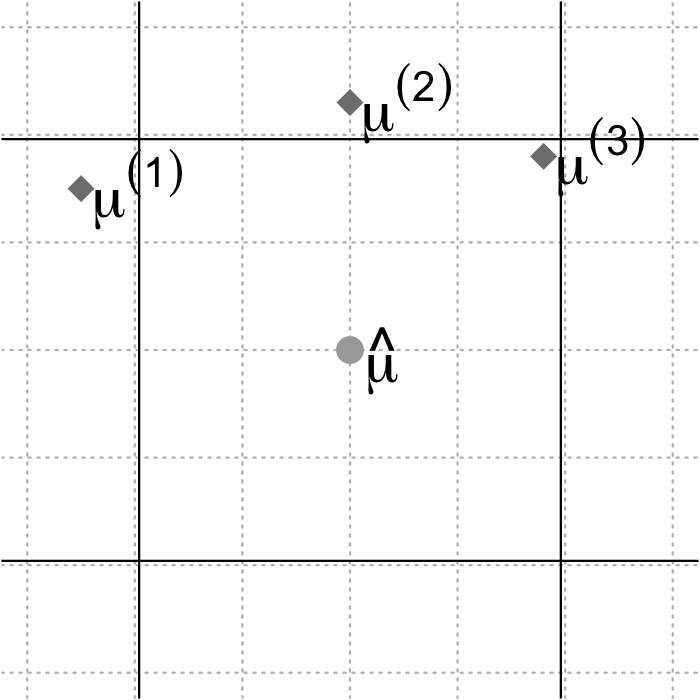
\includegraphics[width = 0.220\textwidth]{./img/intervalsRho0.png} &
%\includegraphics[width = 0.220\textwidth]{./img/ellipseRho0.png} &
%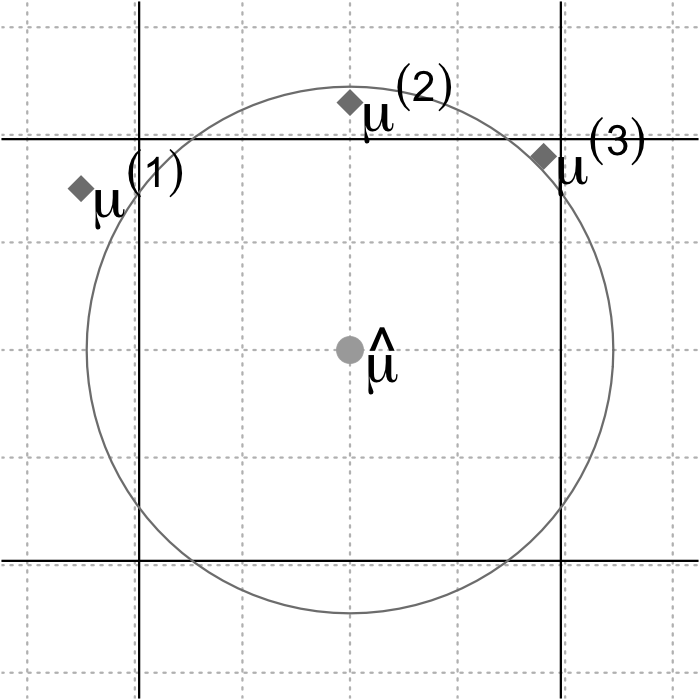
\includegraphics[width = 0.220\textwidth]{./img/intervalsEllipseRho0.png} \\
%{\footnotesize (a) $95\%$ confidence intervals} & 
%{\footnotesize (b) $95\%$ confidence region} &
%{\footnotesize (c) Comparing them} 
%\end{tabular}
%\end{center}
%\caption{Combining multiple $95\%$ confidence intervals versus a single $95\%$ confidence region.  All are centred about $\widehat{\sv{\mu}}$.  In this case $\rho = 0$ and the tests are independent. Grid shows unit squares.}
%\label{fig:confIntervals}
%\end{figure}
%There, the confidence intervals for each coordinate of $\sv{\mu}$ is formed on its margin and drawn as lines parallel to the other axis.  The two vertical lines of Figure \ref{fig:confIntervals}(a) are at the end points of the $95\%$ confidence interval $ [\widehat{\mu}_1 - 1.96,  ~~\widehat{\mu}_1 + 1.96]$ for $\mu_1$; the two horizontal lines are at the endpoints of the $95\%$ confidence interval $ [\widehat{\mu}_2 - 1.96,  ~~\widehat{\mu}_2 + 1.96]$ for $\mu_2$.   
%Consider in turn the hypotheses $H_1: \sv{\mu} = \sv{\mu}^{(1)}$, $H_2: \sv{\mu} = \sv{\mu}^{(2)}$, and $H_3: \sv{\mu} = \sv{\mu}^{(3)}$ and whether they would each be rejected or not at the fixed level $\alpha = 0.05$.  From Figure \ref{fig:confIntervals}(a),  $H_1$ would be rejected because the first coordinate of $ \sv{\mu}^{(1)}$ is outside the confidence interval for $\mu_1$ and $H_2$ would be because the second coordinate of $ \sv{\mu}^{(2)}$ is outside the confidence interval for $\mu_2$.  $H_3$ would be accepted because all of the coordinates of $\sv{\mu}^{(3)}$ are inside their respective confidence intervals; that is, $\sv{\mu}^{(3)}$ is inside the $M$-dimensional box formed by the marginal confidence intervals.
%Contrast these results with the those of the multivariate test, shown again in  Figure \ref{fig:confIntervals}(b). 
%Here,  only $H_2$ would be accepted; both $H_1$ and $H_3$ would be rejected.   The two methods agree only on $H_1$.
%The problem can be seen when we compare the two regions, namely the box formed by the product of the intervals and the circle formed by the joint confidence region.  As  Figure \ref{fig:confIntervals}(c) shows, the areas covered by the two regions is quite different; the box is nearly entirely inside the circle.  The circle was constructed to have an associated probability mass of $1 - \alpha$; the box was not.  For the probability mass to be the same, that associated with the circle cut outside the box would have to match that associated with the corners of the box outside the circle.  On the face of it, and understanding the contours of the probability as indicated in Figure \ref{fig:ellipseAlphas}(a), this cannot be.
Indeed, the probability of rejecting the multivariate hypothesis $H_0$ based on the rejection of one or more of the univariate hypotheses $H_{0i}$ is
\[
\begin{array}{rcl} 
Pr(\mbox{rejecting } H_0 &\given& H_0 ~\mbox{is true} ) \\
&&\\
&=& 
Pr(\mbox{At least one of } H_{01}, H_{02}, \ldots, H_{0M} ~\mbox{is rejected} \given  H_0 ~\mbox{is true} ) \\
&&\\
&=& 
1 - Pr(\mbox{None of } H_{01}, H_{02}, \ldots, H_{0M} ~\mbox{are rejected} \given  H_0 ~\mbox{is true} )
\end{array}
\]
If the tests are independent, that is $\rho_{ij} = 0$ for all $i$, $j$, then 
\[
\begin{array}{rcl} 
Pr(\mbox{rejecting } H_0 \given H_0 ~\mbox{is true} ) &=&
1 - \prod_{i=1}^M Pr(H_{0i}~ \mbox{is not rejected} \given  H_0 ~\mbox{is true} )\\
&&\\
&=& 
1 - \prod_{i=1}^M (1 - \alpha_i)
\end{array}
\]
where the significance level $\alpha_i$ is used to accept or reject $H_{0i}$.  
Supposing that the same significance level,  $\alpha_i = \alpha_{individ}$,  
is used for each individual hypothesis; the experiment-wide significance level is
\begin{equation}
\begin{array}{rcl} 
\alpha = Pr(\mbox{rejecting } H_0 \given H_0 ~\mbox{is true} ) = 
1 -  (1 - \alpha_{individ})^M.
\end{array}
\label{eq:multipleTesting:alphaExperiment}
\end{equation}
% For the example of Figure \ref{fig:confIntervals}(c), where $\alpha_{individ} = 0.05$ and $M = 2$, Equation (\ref{eq:alphaExperiment}) shows that the  experiment-wide significance level of the test is actually $\alpha = 0.0975$.
This introduces an inflated type one error when using multiple independent tests. In the case where $M=2$, $\rho = 0$, and $\alpha_{individ} = 0.05$, the joint hypothesis $H_0$ will be rejected $9.75\%$ of the time when $H_0$ is true, rather than the putative $5\%$ of the time. These individual tests produce more false positives than the $5\%$ planned. Alternatively, as a confidence region for $\sv{\mu}$, the box defined by these marginal tests has an associated confidence level of $(1 - \alpha_{individ})^M$ rather than $1 - \alpha$. %In the example, this means the box as confidence region in Figure \ref{fig:confIntervals}(c) has coverage of only $90.25\%$ compared to the $95\%$ coverage by the circle.  

\subsection{Accounting for multiple tests}

One way to still use the confidence intervals, or equivalently the independent tests, is to adjust the significance levels for each individual test to get the desired significance level for their combination. Turning Equation (\ref{eq:multipleTesting:alphaExperiment}) around and solving for $\alpha_{individ}$ gives
\begin{equation}
\alpha_{individ} = 1 - (1 - \alpha)^\frac{1}{M}.
\label{eq:multipleTesting:adjIndep}
\end{equation}
This indicates that for an experiment-wide significance level of $\alpha$, each of the $M$ individual significance levels should be adjusted to be the value $\alpha_{individ}$ from Equation (\ref{eq:multipleTesting:adjIndep}) and the critical value $c_{\alpha_{individ}}$ determined accordingly.   

%Figure \ref{fig:confIntervalsCorrected}(a)
%\begin{figure}[htp]
%\begin{center}
%\begin{tabular}{ccc}
%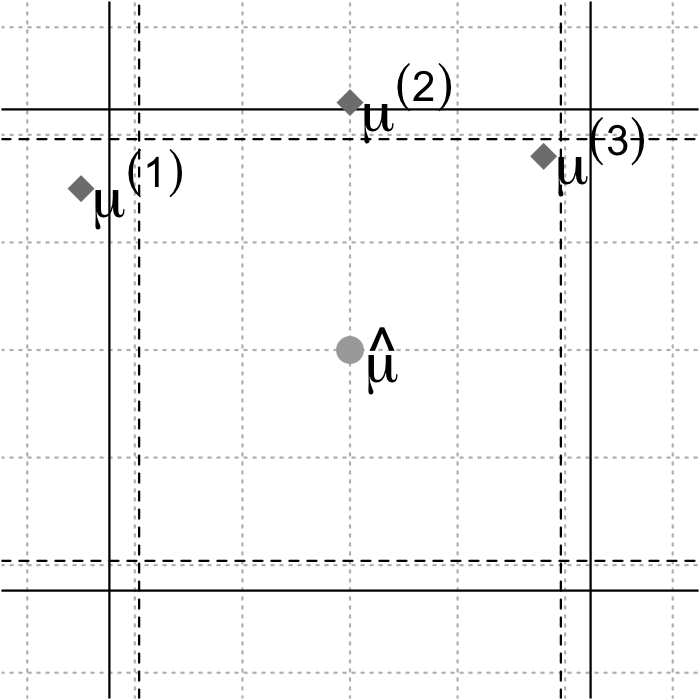
\includegraphics[width = 0.220\textwidth]{./img/intervalsCorrectedRho0.png} &
%\includegraphics[width = 0.220\textwidth]{./img/ellipseRho0.png} &
%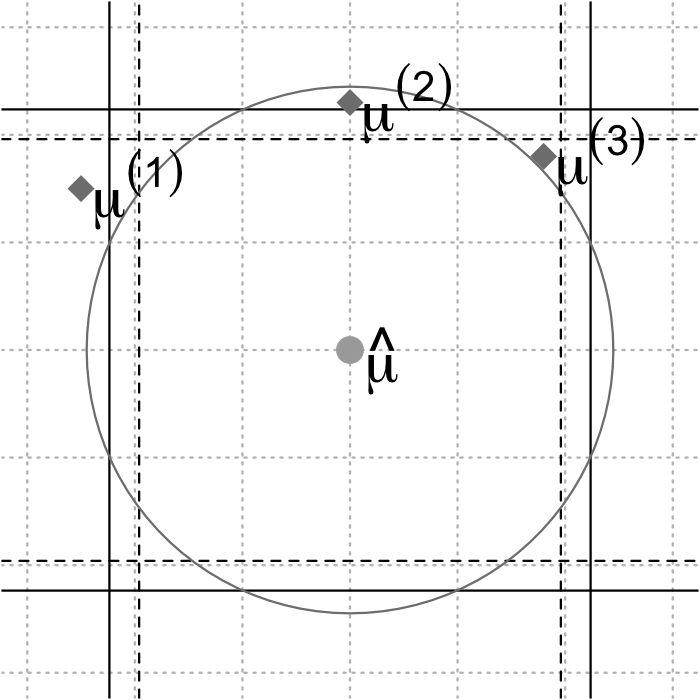
\includegraphics[width = 0.220\textwidth]{./img/intervalsCorrectedEllipseRho0.png} \\
%{\footnotesize (a) Solid line box is a $95\%$ } & 
%{\footnotesize (b) $95\%$ confidence region} &
%{\footnotesize (c) Comparing them} 
%\\
%{\footnotesize  confidence region} &  &
%\end{tabular}
%\end{center}
%\caption{Combining multiple confidence intervals versus a single confidence region.  Corrected intervals are solid lines ($\alpha_{individ} = 0.02532057$); uncorrected are dashed ($\alpha_{individ} = 0.05$).  Grid shows unit squares.}
%\label{fig:confIntervalsCorrected}
%\end{figure}
%shows the box from the corrected intervals as solid lines and the uncorrected as dashed lines.  The correction makes the box larger so that its coverage probability is now $95\%$.  In Figure \ref{fig:confIntervalsCorrected}(c) the expanding box has produced larger corners outside the circle and cut smaller parts of the circle off.  The Cartesian area of the corners is larger than that of the circle pieces outside the box so that the probability mass associated with these areas match.

Note that these adjusted multiple tests and the multivariate test are matched only on their fixed significance level $\alpha$ or coverage probability $1 - \alpha$. The multiple tests only use marginal distributions whereas the multivariate test uses the joint distribution. Consequently, they may still disagree on which hypotheses to accept and which to reject, %(see Figure \ref{fig:confIntervalsCorrected}(c))
though this will occur less often than with the unadjusted test.

Sometimes, an even simpler adjustment commonly called a \emph{Bonferroni correction} is made. Instead of using Equation (\ref{eq:multipleTesting:adjIndep}), simply choose
\begin{equation}
\alpha_{individ} = \frac{\alpha}{M}.
\label{eq:multipleTesting:adjIndepApprox}
\end{equation}
%or $0.025$ instead of $0.02532057$ from Figure  \ref{fig:multipleTesting:confIntervalsCorrected}.
For small $\alpha$ and large $M$, this is very nearly the same value as in Equation (\ref{eq:multipleTesting:adjIndep}) since $(1 - \alpha)^\frac{1}{M} \approx 1 - \frac{\alpha}{M}$.  It is easier to remember in any case.

\subsection{Dependent multiple tests}
The problem is that the marginal tests are {\bf not} independent whenever $\sm{\Sigma} \ne \m{I}_M$, and so Equation (\ref{eq:multipleTesting:adjIndep}) does not strictly apply.
Figure \ref{fig:multipleTesting:confIntervalsCorrectedRho}
\begin{figure}[htp]
\begin{center}
\begin{tabular}{cccc}
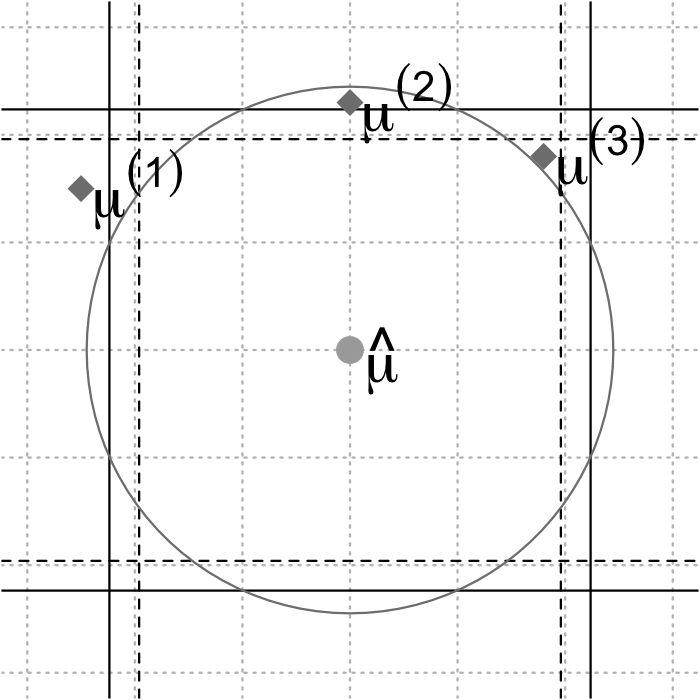
\includegraphics[width = 0.220\textwidth]{./img/intervalsCorrectedEllipseRho0.png} &
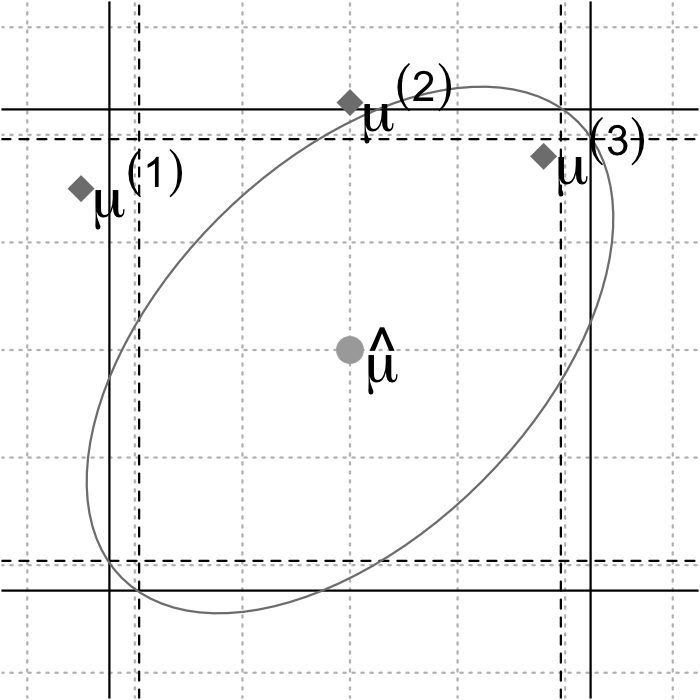
\includegraphics[width = 0.220\textwidth]{./img/intervalsCorrectedEllipseRho5.png} &
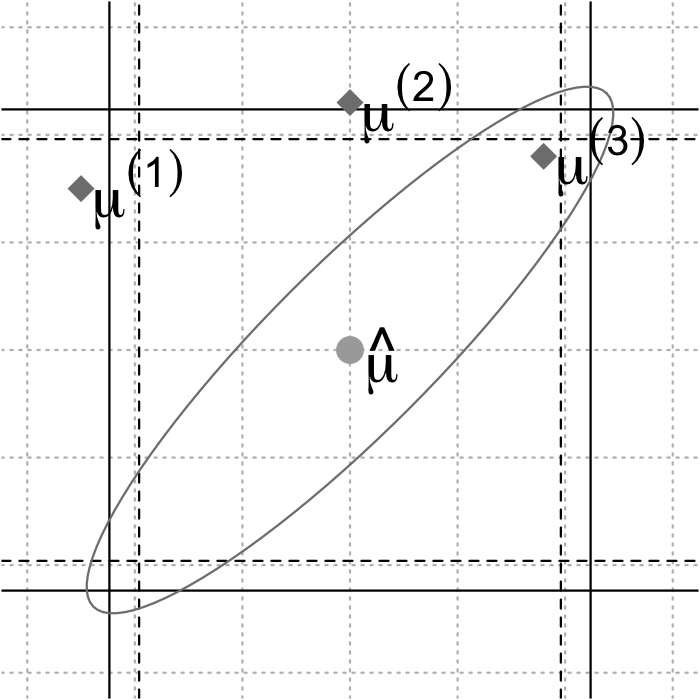
\includegraphics[width = 0.220\textwidth]{./img/intervalsCorrectedEllipseRho9.png} &
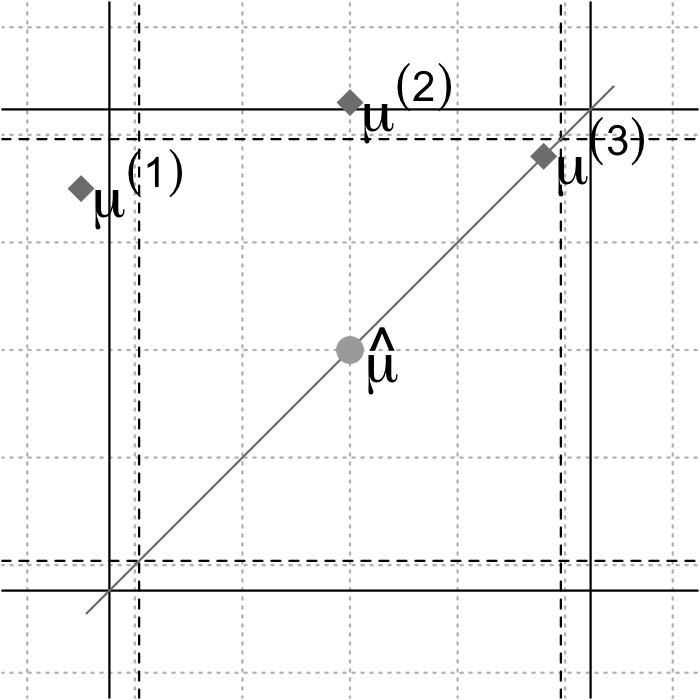
\includegraphics[width = 0.220\textwidth]{./img/intervalsCorrectedEllipseRho10.png} 
\\
{\footnotesize  (a) Independent tests } &  
{\footnotesize  (b) Dependent tests }&
{\footnotesize  (c) Dependent tests } &
{\footnotesize  (d) Dependent tests } 
\\
{\footnotesize $\rho = 0$ } & 
{\footnotesize $\rho = 0.5$} &
{\footnotesize $\rho = 0.9$} &
{\footnotesize $\rho = 1.0$} 
\end{tabular}
\end{center}
\caption{Combining multiple confidence intervals versus a single $95\%$confidence region for varying $\rho$.  Corrected intervals are solid lines ($\alpha_{individ} = 0.025$); uncorrected are dashed ($\alpha_{individ} = 0.05$).   Grid shows unit squares.}
\label{fig:multipleTesting:confIntervalsCorrectedRho}
 \end{figure}
compares the corrected and uncorrected intervals for $M = 2$ and different values of $\rho$, the correlation between the marginal tests. In each of Figures \ref{fig:multipleTesting:confIntervalsCorrectedRho}(a), (b), (c), and (d), the coverage probability of the ellipse is 0.95,  the correct value for $\alpha = 0.05$. Table \ref{tab:multipleTesting:coverage}
\begin{table}[htp]
\begin{center}
\begin{tabular}{c|cccc}
& 
$\rho = 0$ &
$\rho = 0.5$ &
$\rho = 0.9$&
$\rho = 1.0$ \\
\hline
Uncorrected & 
0.902 (0.098) &
0.909 (0.091) &
0.930 (0.070) &
0.950 (0.050)
\\
Corrected &
0.950 (0.050) &
0.953 (0.047) &
0.963 (0.037) &
0.975 (0.025)

\end{tabular}
\end{center}
\caption{Coverage probabilities and experiment-wide $\alpha$ levels for boxes defined by multiple marginal test intervals.}
\label{tab:multipleTesting:coverage}
\end{table}
gives the coverage probabilities (and experiment wide $\alpha$ levels in parentheses) for the boxes defined by the multiple test intervals of Figures \ref{fig:multipleTesting:confIntervalsCorrectedRho}(a), (b), and (c).  
These are correct in only two cases. The case $\rho = 0$ is that for which the correction was designed and $\alpha_{individ}$ was set correctly. When $\rho = 1$,  all probability mass lies only along the box diagonal and all marginal tests will reject whenever one does. More generally, as $\rho$ increases, the ellipses narrow and the probability concentrates nearer the box diagonal. As a consequence, the probability mass covered by either box increases. The correction, designed for independent tests, is no longer correct when tests are dependent.

When the tests are not independent, it has been suggested that the adjustment given by Equation (\ref{eq:multipleTesting:adjIndep}), or by Equation (\ref{eq:multipleTesting:adjIndepApprox}), still be used but that the number of independent tests $M$ be replaced by some measure of the \emph{effective number} of independent tests. That is, the adjustments become
\begin{equation}
\alpha_{individ} = 1 - (1 - \alpha)^\frac{1}{M_{eff}}
\label{eq:multipleTesting:adjIndepEff}
\end{equation}
or simply
\begin{equation}
\alpha_{individ} = \frac{\alpha}{M_{eff}}
\label{eq:multipleTesting:adjIndepEffApprox}
\end{equation}
for the Bonferroni correction. $M_{eff}$ is now some measure of the effective number of independent tests, and so need not necessarily be an integer.

\subsection{Variance of the Eigenvalues}

The first suggested adjustment was that given by \cite{cheverud2001} based on the sample variance $V_\lambda$  of the eigenvalues of the correlation matrix $\sm{\Sigma}$, namely
\[ V_\lambda = \frac{\sum_{i=1}^M (\lambda_i - 1)^2}{M-1}. \]
This variance has been interpreted by \cite{cheverud2001} as a measure of the ``total correlation'' among the set of ``traits'' or tests defining $\sm{\Sigma}$. When all are independent then $\sm{\Sigma} = \m{I}_M$ and $V_\lambda = 0$, its minimum value; when all are maximally correlated, $\rho_{ij} = 1$ for all $i \ne j$ and $V_\lambda = M$, its maximum value. The ratio $\left( V_\lambda / M \right)$ varies from its minimum 0 when there are $M$ independent tests to its maximum 1 when there is essentially 1 test since they are maximally correlated. A simple location scale change of the ratio $\left( V_\lambda / M \right)$ from $[0,1]$ to $[M, 1]$ suggests using
\begin{equation}
M_{eff} = M - (M-1) \frac{V_\lambda}{M} %= 1 + (M-1)\left(1 - \frac{V_\lambda}{M} \right)
\label{eq:multipleTesting:meff_var}
\end{equation}
as the effective number of tests. This is the expression used in \cite{nyholt2004}.

If $M_{eff}$ is used in place of $M$ in the correction formula as in Equation (\ref{eq:multipleTesting:adjIndepEff}), the following table
\begin{table}[htp]
\begin{center}
\begin{tabular}{c|cccc}
& 
$\rho = 0$ &
$\rho = 0.5$ &
$\rho = 0.9$ &
$\rho = 1.0$ \\
\hline
$M_{eff}$ & 
2 &
1.75 &
1.19 &
1
\\
Coverage  &
0.950 &
0.947 &
0.940  &
0.950 
\\
$\alpha$  &
0.050 &
0.053 &
0.060 &
0.050

\end{tabular}
\end{center}
\caption{Coverage probabilities and experiment-wide $\alpha$ levels for boxes adjusted by $M_{eff}$ from \cite{cheverud2001}.}
\label{tab:multipleTesting:coverageMvar}
\end{table}
results for the cases illustrated in Figure \ref{fig:multipleTesting:confIntervalsCorrectedRho}.  As can be seen, the correction, the coverage, and the $\alpha$ are correct for the two end cases when $\rho = 0$ and $\rho = 1$.  In between, the effective number of cases is a real number between one and two, increasing in size as the correlation moves toward zero.  In these between cases, the coverage probability (or $\alpha$) is fairly close to its target value of $0.95$ (or $0.05$).

In terms of the eigenvalues Equation (\ref{eq:multipleTesting:meff_var}) can be rewritten as 
\begin{equation}
M_{eff} = M + 1 - \frac{\sum_{i=1}^M \lambda_i^2}{M}. %= 1 + (M-1)\left(1 - \frac{V_\lambda}{M} \right)
\label{eq:multipleTesting:meffeigen}
\end{equation}
In the special case where $\rho_{ij} = \rho $ for all $i \ne j$, then $V_\lambda = M\rho^2$ and
\begin{equation}
M_{eff} = M - (M-1) \rho^2.
\label{eq:multipleTesting:meffeigenSpecialRho}
\end{equation}
Two edge cases are often considered: the independent case when $\rho = 0$ and the maximally correlated case when $\rho = 1$. In the first of these $M_{eff} = M$ as it should. When $\rho = 1$, it is as if the same test has been applied $M$ times and $M_{eff} = 1$ correctly reflects that only a single test has been applied.

Similarly, we could imagine $m$ copies of $k$ independent tests. This would amount to a block diagonal $(mk) \times (mk)$ matrix $\sm{\Sigma}$ having $k$ identical $m \times m$ matrices of ones down the diagonal and zeros elsewhere\footnote{A similar block diagonal structure is natural in genetic studies.}. The resulting eigenvalues are $\lambda_1 = \cdots = \lambda_k = m$ and $\lambda_{k+1} = \cdots = \lambda_M = 0$, where $M = km$.  The number of independent tests here is clearly $k$. Unfortunately, in this case Equation (\ref{eq:multipleTesting:meffeigen}) gives
\begin{equation}
M_{eff}  =  km + 1 - \frac{km^2}{km} = (k-1)m +1 
\label{eq:multipleTesting:Meff_varIndepTestCopies}
\end{equation}
which equals $k$ only when $m = 1$, and is larger otherwise.

When there are differing numbers $m_1 > m_2 > \cdots > m_k \ge1$ of the $k$ tests, then again Equation (\ref{eq:multipleTesting:meffeigen}) leads to 
\[
M_{eff}  =  M + 1 - \frac{\sum_{i = 1}^k m_i^2}{M}  
\]
where $M = \sum_{i = 1}^k m_i$.  Again this will be very different from $k$.

Considerations of cases such as these have led \cite{LiJi2005} to an alternative proposal for $M_{eff}$ which will return $k$ in both cases.

\subsection{Separating Integral and Fractional Contributions}

Noting the counter-intuitive behaviour of $M_{eff}$ revealed in Equation (\ref{eq:multipleTesting:Meff_varIndepTestCopies}) when independent tests are copied multiple times each, \cite{LiJi2005} craft a new proposal based entirely on the eigenvalues. They suggest that each eigenvalue $\lambda_i $ be separated into two parts, its integral part ($\ge 1$) and its fractional remainder. Its integral part counts as a single independent test and its fractional part as a ``partially correlated test'' to be counted as some fraction between 0 and 1.

Mathematically, this amounts to a function $g(x)$ 
defined as 
\begin{equation}
g(x) = I _{[1, \infty)} (\lambda_i) +  f_i
\end{equation}
where $I_A(x)$ is the usual indicator function and $f_i = \lambda_i - \lfloor \lambda_i \rfloor$ is the fractional remainder after removing the floor function $\lfloor \cdot \rfloor$.   Note that \cite{LiJi2005} imagine cases where $\sm{\Sigma}$ possibly has negative eigenvalues\footnote{This situation will arise if the elements of $\sm{\Sigma}$ have been separately determined without constraint that $\sm{\Sigma}$ satisfy the definition of a correlation matrix and hence be non-negative definite. In many genetic surveys, this is the reality of the correlations measured.}. In that case, they replace $\lambda_i$ by $\abs{\lambda_i}$ everywhere. A better solution might instead be to replace $\sm{\Sigma}$ by its nearest non-negative definite matrix approximation before continuing. \TODO{Justify this statement, seems like the crux of the justification is that the hypersphere of the nearest non-negative definite matrix would better approximate the true coverage region}

Following this intuition, \cite{LiJi2005}  propose  $M_{eff}$ be replaced by
\begin{equation}
 M_{eff}^*  = \sum_{i=1}^M g(\lambda_i) 
\label{eq:multipleTesting:meff_frac}
\end{equation}
in place of the original by \cite{cheverud2001} shown in Equations (\ref{eq:multipleTesting:meff_var}) and (\ref{eq:multipleTesting:meffeigen}).

Like the definition of Equation (\ref{eq:multipleTesting:meff_var}), this returns $M^*_{eff} = 1$  and $M_{eff}^* = M$ for the edge cases of $M$ maximally correlated tests and $M$ independent tests, respectively. It also addresses the problems raised for the cases where $k$ independent tests are repeated $m$ times each. $M_{eff}^* = k$ no matter how many times each of the $k$ independent tests were repeated.

Applying  $M^*_{eff}$ to the examples of Figure \ref{fig:multipleTesting:confIntervalsCorrectedRho} gives the results shown in Table \ref{tab:multipleTesting:coverageMfrac}.
\begin{table}[htp]
\begin{center}
\begin{tabular}{c|cccc}
& 
$\rho = 0$ &
$\rho = 0.5$ &
$\rho = 0.9$ &
$\rho = 1.0$ \\
\hline
$M_{eff}^*$ & 
2 &
2 &
2 &
1
\\
Coverage  &
0.950 &
0.953 &
0.963  &
0.950 
\\
$\alpha$  &
0.050 &
0.047 &
0.037 &
0.050
\end{tabular}
\end{center}
\caption{Coverage probabilities and experiment-wide $\alpha$ levels for boxes adjusted by $M_{eff}^*$ from \cite{LiJi2005}.}
\label{tab:multipleTesting:coverageMfrac}
\end{table}
Careful examination of these results reveals a new peculiarity with this definition. In the case when $M=2$, $M_{eff}^* = 2$ for any $\rho < 1$ and the resulting intervals are necessarily uncorrected!

The problem is that the equal correlation structure of Equation (\ref{eq:multipleTesting:commonCor}) gives $\lambda_1 = 1 + (M-1)\rho$ and $\lambda_2 = \cdots = \lambda_M = 1- \rho$. For $\rho \ge 0$, $\lambda_1 \ge 1$ and its fractional remainder is $f_1 = (M-1)\rho - \lfloor (M-1)\rho \rfloor$. The remaining $\lambda_i  = f_i = 1 - \rho < 1$ for all $i \ne 1$.

For  $\rho \ge 0$, then, 
\begin{eqnarray}
M_{eff}^* &=&  1 + f_1+ (M-1)(1-\rho) 
\nonumber \\
&& \nonumber \\
&=& M - \lfloor (M-1) \rho \rfloor.
\label{eq:multipleTesting:meff_fracstep}
\end{eqnarray}
When $M=2$, $M_{eff}^* = 2$ no matter what value $\rho < 1$ takes and so no correction is made. The values for the two edge cases are also easily derived from this equation: when $\rho =0$, $M_{eff}^*= M$; when $\rho =1$, then $M_{eff}^*=1$. 

Note also from Equation (\ref{eq:multipleTesting:meff_fracstep}), that $M_{eff}^*$ takes only integer values and is a step function of $\rho$. The value of $M_{eff}^* = M- k$ is constant for all $\rho \in [\frac{k}{M-1},  \frac{k+1}{M-1} )$ with each non-negative integer $k \le M-2$.  The smaller is $M$, the wider is the range of $\rho$ returning an identical value for $M_{eff}^*$.  For example, when $M=3$, all values of $\rho \in [0, 0.5) $ return  $M_{eff}^* = 3$.

In the unusual case where $-1/(M-1) \le \rho < 0$ (i.e. $\sm{\Sigma}$ remains a correlation matrix), the largest eigenvalue will be $1- \rho = 1 +\abs{\rho}$ in this instance, and there will be $M-1$ copies of this.
The single smaller eigenvalue will be $ 1 - (M-1)\abs{\rho}$ which is a positive fraction $f_M$ since $\abs{\rho} \le 1/(M-1)$.  Together, in the case where $-1/(M-1) \le \rho < 0$, these results give
\[
\begin{array}{rcl}
M_{eff}^* &=&  (M-1) \times 1 + (M-1) \abs{\rho} + f_M  \\
&&\\
&=&  (M-1)(1 + \abs{\rho}) + (1 - (M-1)\abs{\rho}) \\
&&\\
&=&  M
\end{array}
\]
independent of whatever value $\rho$ takes, provided it is negative.  Whatever value $\rho < 0$ takes, provided it is negative, no correction will be made using $M_{eff}^*$.  

In contrast, under the same conditions, $M_{eff}$ of \cite{cheverud2001} is symmetric in $\rho$ about $0$ according to Equation (\ref{eq:multipleTesting:meffeigenSpecialRho}) provided $\abs{\rho} \le 1/(M-1)$.   One could argue that this is the sensible choice.  Small values of $\abs{\rho}$ indicate $M$ nearly, but not quite,  independent tests.  It seems unusual to treat the multiple marginal tests as if they are dependent when $\rho >0$ but as if they are independent when $\rho < 0$, yet this is exactly what $M_{eff}^*$ does.

%\comment{It may be the case that $M_{eff}^*$ performs better for large $M$ than it does for small $M$.}

%\TODO{

%Plot $M_{eff}$ and $M_{eff}^*$ as $M$ increases for varying values of $\rho$.

%Weird for other special cases too.  Including, I think, for the motivating case. If $\lambda_i = \frac{M}{k}$ for $ i = 1, \ldots, k$ and $\lambda_i = 0$ for $i  > k$, then $M_{eff} > k$ except when $k = 1$. }

\subsection{Effective Dimension}

A final approach is motivated by the shape of the confidence ellipsoids as determined by the relative lengths of their principal axes. For example, when $M = 2$, various confidence ellipses are shown in Figure \ref{fig:multipleTesting:confIntervalsCorrectedRho} to demonstrate the change probability mass and so how the box formed by the separate multiple tests must change to match it.

When $M = 2$, a rotated ellipse appears as in Figure \ref{fig:multipleTesting:ellipseAxes}. 
\begin{figure}[htp]
\begin{center}
\begin{tabular}{cp{0.5\textwidth}}
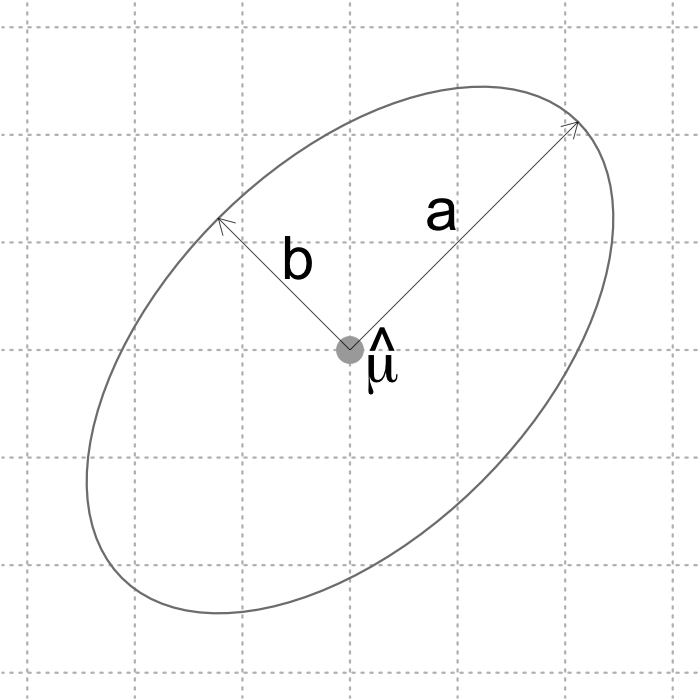
\includegraphics[width = 0.30\textwidth]{./img/ellipseAxesRho5.png} &
\vspace{-0.2\textheight}
{\footnotesize
Once rotated, the equation of this ellipse in two dimensions is:
 \[
\frac{x^2}{a^2} + \frac{y^2}{b^2}  = 1
\]
Setting $x = 0$, solve for the limits for $y$ to give $\pm \sqrt{a}$.
Similarily, set $y =0$ to give limits of $x$ as $\pm \sqrt{b}$}
%{\footnotesize $\rho = 0.5$} \\
%{\footnotesize $\alpha = 0.05$}
\end{tabular}
\end{center}
\caption{The major and minor semi-axes of the $95\%$ confidence ellipse centred at $\widehat{\sv{\mu}}$ when $M =2$,  $\rho = 0.5$, and $\alpha = 0.05$.  Lengths are marked as $a$ and $b$.   Grid shows unit squares.}
\label{fig:multipleTesting:ellipseAxes}
\end{figure}
As can be seen, the lengths of the principal semi-axes are easily determined, giving $a = \sqrt{ C_\alpha  \lambda_1}$ and $b = \sqrt{ C_\alpha \lambda_2}$. Note that $C_\alpha$ changes the length depending on the size of $\alpha$ and so does not depend on the underlying correlation structure. Whatever the choice of $\alpha$ the major and minor axes will have lengths proportional to $\sqrt{\lambda_1}$ and $\sqrt{\lambda_2}$, respectively. That is, the shape of the ellipse is determined entirely from the eigenvalues of the correlation matrix.

In some sense, each eigenvalue gives the support for the existence of a dimension along that axis. When one of them is zero, the axis and dimension associated with that value disappears as in Figure \ref{fig:multipleTesting:confIntervalsCorrectedRho}(c).

For $M$-dimensional data, there will be $M$ such semi-axes of Euclidean length $\sqrt{\lambda_i}$ on the $i$ the axis. A formal definition given by \cite{oldford1987n} is that the \emph{effective dimensionality} could be measured by the function
\[
d(\lambda_1, \cdots, \lambda_M; p) = \sum_{i = 1}^M  \left( \frac{\lambda_i}{\lambda_{max}}\right)^{p} = \sum_{i = 1}^M  \left( \frac{\lambda_i}{\lambda_1}\right)^{p}
\]
for any choice of $p \in [0, \infty)$, where different choices of $p$ may be fit for different purposes.  The smaller each $\lambda_i \ge 0$ is compared to the $\lambda_{max} = \lambda_1 > 0$, the less relative support there is for that dimension.

The parameter $p$ determines the rate at which the contribution of the shorter directions to the effective dimension are attenuated.  When $p = 0$,  $d_p$ simply counts the number of non-zero $\lambda_i$s and so returns the rank of $\sm{\Sigma}$ as the dimension. As $p$ increases, the contribution of the shorter minor axes diminishes, eventually reaching zero as $p \rightarrow \infty$ at which point $d_p$ simply counts the number of equivalent major axes of the ellipsoid. The minimal effective dimension is 1 and the maximum is $M$ for all $p \in [0, \infty)$.

For the multiple testing problem, the attenuation must not be so sharp that it throws away independent tests. One might choose $p = (1/M)$ so that the effective number of tests is estimated by the effective dimension using the $M$th root of the eigenvalues. That is, 
\begin{equation}
M_{eff}^{**} = \sum_{i = 1}^M  \left( \frac{\lambda_i}{\lambda_{max}}\right)^{1/M}
\label{eq:multipleTesting:meff-ED}
\end{equation}
This choice is motivated, in part, by considering the problem of simply repeatedly adding same test over and over to a bank of tests.

For example, suppose $\sm{\Sigma}$ is a block diagonal matrix
\begin{equation}
\sm{\Sigma} = \left[ \begin{array}{cc}
                                \sm{\Sigma}_{11} & \m{0} \\
                                \tr{\m{0}} &  \sm{\Sigma}_{22} 
                                \end{array}
                        \right]
\label{eq:multipleTesting:block-diagonal}
\end{equation}
where the $m_1 \times m_1$ matrix $\sm{\Sigma}_{11}$ and the $m_2 \times m_2$ matrix $\sm{\Sigma}_{22}$ are both correlation matrices with $M = m_1 + m_2$.  These two matrices  represent separate independent groups of tests since all correlations between the two groups are zero as shown by the $m_1 \times m_2$ off-diagonal zero-matrix, denoted by $\m{0}$. 

Suppose each of $\sm{\Sigma}_{11}$ and  $\sm{\Sigma}_{22}$ have the common correlation structure of Equation (\ref{eq:multipleTesting:commonCor}) but with different correlations $\rho_{11} \ge 0$ and $\rho_{22} \ge 0$.  The eigenvalues of $\sm{\Sigma}$ are then $(m_1 - 1)\rho_{11} +1$, $(m_2 - 1)\rho_{22} +1$, $(1 - \rho_{11})$ repeated $(m_1 -1)$ times, and $(1 - \rho_{22})$ repeated $(m_2 -1)$ times.  Which is the largest eigenvalue will depend on the values of  the pairs $m_1$, $\rho_{11}$,  and $m_2$,  $\rho_{22}$; when $\rho_{11} = \rho_{22}$, for example, the largest eigenvalue belongs to the largest group. 

To see the effect of increasing $M$, consider the case when $\rho_{22} = 0$ but $\rho_{11} \ne 0$.  The $m_2$ tests in the second group are independent with unit eigenvalues and the $m_1$ tests in the first group are dependent with eigenvalues as above.   
The effective dimension for any $p$ becomes
\begin{equation}
d(\lambda_1, \cdots, \lambda_M; p) = 1 
       + \frac{m_2}{ \left(1 + (m_1 - 1) \rho_{11}\right)^p}
       + (m_1 - 1) \left( 
               \frac{1- \rho_{11}}
                      {1 + (m_1 - 1) \rho_{11}}  
                 \right)^p.
\label{eq:multipleTesting:EDblockIndep}
\end{equation}  
When either $m_1 = 1$ or $\rho_{11} = 0$  also holds, then the effective dimension is $M = m_1 + m_2$, as it should be for $M$ independent tests.

However, when this is not the case, the contribution of the $m_2$ can be made arbitrarily small for fixed $p$ by simply increasing $m_1$. The contribution from the second group of independent tests lies entirely with the second term of 
Equation (\ref{eq:multipleTesting:EDblockIndep}) while that of the first group is spread over the second and third terms. Increasing $m_1$ will not only increase the contribution of the first group in the third term but it will also \emph{decrease} the second group's contribution!  

This effect is perhaps most dramatic, as well as most worrying, when $\rho_{11}$ is maximal, that is $\rho_{11} = 1$.  Then
\[
d(\lambda_1, \cdots, \lambda_M; p) = 1 + m_2 \left(\frac{1}{ m_1} \right)^p
\]
and simply increasing $m_1$ can entirely remove the effect of the second group of independent tests.
When $\rho_{11} = 1$ is maximal, then the $m_1$ tests in the first group are effectively the same test.  
By simply repeating the same test $m_1$ times, achieving the same answer each time, the contribution of the $m_2$ independent tests can be effectively obliterated!

Looking again at the second term in Equation (\ref{eq:multipleTesting:EDblockIndep}), the ideal solution in this case would have the denominator be equal to one.  As a function of $m = m_1$ and $p$ this denominator behaves roughly like 
\[(1 + m)^p.\]
For fixed $m$, the smaller is $p$, the closer this is to one.  For fixed $p$, the larger is $m$, the farther this moves from one, getting larger and larger.  The obvious solution is to choose $p = 1/m$, for then one corrects the other and  $\lim_{m \rightarrow \infty} (1 + m)^{1/m} = 1$.

This suggests the choice $ p = 1/M$ in general; all limits still hold since $M = m_1 + m_2$ (including the original denominator going to 1). Moreover, this choice amplifies small ratios of $\frac{\lambda_i}{\lambda_{max}}$ more as $M$ increases.  This choice leads to
\[
M_{eff}^{**} = \sum_{i = 1}^M  \left( \frac{\lambda_i}{\lambda_{max}}\right)^{1/M}
\]
as suggested earlier.

Each $\lambda_i$ is proportional to the Euclidean length of a principal axis of the confidence ellipsoid determined by $\sm{\Sigma}$ with proportionality constant determined by the choice of $\alpha$.  Ratios of axis lengths remove the proportionality constant allowing the effective number of tests to be independent of the selected significance level $\alpha$.

As with the other choices of  the effective number of tests $M_{eff}^{**}$, we can examine the coverage probabilities for $M_{eff}^{**}$ defined as the effective dimensionality of Equation (\ref{eq:multipleTesting:meff-ED}) for the cases of Figure \ref{fig:multipleTesting:confIntervalsCorrectedRho}. The results are given
in the table below.
\begin{center}
\begin{tabular}{c|cccc}
& 
$\rho = 0$ &
$\rho = 0.5$ &
$\rho = 0.9$ &
$\rho = 1.0$ \\
\hline
$M_{eff}^{**}$ & 
2 &
1.57735 &
1.229416 &
1
\\
Coverage  &
0.950 &
0.941&
0.942 &
0.950 
\\
$\alpha$  &
0.050 &
0.059 &
0.058 &
0.050
\end{tabular}
\end{center}
Similar to the other methods, it agrees in the effective number of tests and gets the coverage probabilities exactly right for the extreme cases of $\rho = 0$ and $\rho = 1$.  The $M$th  root effective dimension is similar to the original proposal by \cite{cheverud2001} in coverage probabilities and in effective number of tests being non-integral for  these examples.  It differs from the indicator function and fractional part method of \cite{LiJi2005} which, for any values of $\rho \in (0,1)$,  has  $M_{eff}^{**} = M = 2$ and so simply reproduces the original independent tests adjustment in terms of effective number of tests and coverage probability (or experiment-wide significance level).

Although not introduced in terms of effective dimension, \cite{Galwey2009} proposes a similar measure in
\begin{equation}
  M_{eff}^{***} = \frac{ \left ( \sum_{i=1}^M \sqrt{\lambda_i} \right )^2}{\sum_{i=1}^M \lambda_i}
  \label{eq:multipleTesting:galwey}
\end{equation}
which is simply the ratio
$$\frac{d(\lambda_1, \cdots, \lambda_M; 1/2)^2}{d(\lambda_1, \cdots, \lambda_M; 1)}.$$


%\section{Comparisons of the Three Methods}

%\subsection{On the Effective Number of Tests}

% \TODO{As a function lambdas, rho, etc for a bunch of different cases.  Entirely via plots.}
 
%Figure \ref{fig:equalEigenValues} 
%\begin{figure}[htp]
%\begin{center}
%\begin{tabular}{cc}
%\includegraphics[width = 0.45\textwidth]{./img/equalEigenValsm10kvary.png} &
%\includegraphics[width = 0.45\textwidth]{./img/equalEigenValsm10kvaryZoom.png} \\
%{\footnotesize (a) As a function of $k$} &
%{\footnotesize (b) As a function of $k$} \\
%{\footnotesize ($k$ is the number of independent tests)} &
%{\footnotesize (zoomed in on vertical axis)} \\
%\includegraphics[width = 0.45\textwidth]{./img/equalEigenValsmvaryk10.png} &
%\includegraphics[width = 0.45\textwidth]{./img/equalEigenValsmvaryk10Zoom.png} \\
%{\footnotesize (c) As a function of $m$} &
%{\footnotesize (d) As a function of $m$ } \\
%{\footnotesize ($m$ is the number of repetitions of each test)} &
%{\footnotesize (zoomed in on vertical axis)} \\
%\end{tabular}
%\end{center}
%\caption{{\bf Repeated independent tests.} 
%Shows the actual experiment wide $\alpha$-level for each method as a function of  the number of independent tests $k$, each repeated $m = 10$ times (top row) or as a function of the number of repetitions $m$, for each of $k = 10$ independent tests (bottom row). Right column is the same as the left but zoomed in on the smaller experiment-wide actual $\alpha$-levels. For all plots the target $\alpha$-level was $\alpha = 0.05$. }
%\label{fig:equalEigenValues}
%\end{figure}
%\comment{From Figure \ref{fig:equalEigenValues} note that only  Meff\_frac  and Meff\_dMinv get the correct experiment wide $\alpha$ level.  Note also that Meff\_frac was designed specifically to address this problem.}



%Figure \ref{fig:equalCorrelationsM} 
%\begin{figure}[htp]
%\begin{center}
%\begin{tabular}{cc}
%\includegraphics[width = 0.45\textwidth]{./img/equalCorRho2.png} &
%\includegraphics[width = 0.45\textwidth]{./img/equalCorRho8.png} \\
%{\footnotesize (a) As a function of $M$; $\rho = 0.2$} &
%{\footnotesize (b) As a function of $M$; $\rho = 0.8$} \\
%\multicolumn{2}{c}{
%\begin{tabular}{ccc}
%\includegraphics[width = 0.3\textwidth]{./img/equalCorRho2Zoom.png} &
%\includegraphics[width = 0.3\textwidth]{./img/equalCorRho5Zoom.png} &
%\includegraphics[width = 0.3\textwidth]{./img/equalCorRho8Zoom.png} \\
%{\footnotesize (c) $\rho = 0.2$ zoomed in} &
%{\footnotesize (d) $\rho = 0.5$ zoomed in} &
%{\footnotesize (e) $\rho = 0.8$ zoomed in} 
%\\

%\end{tabular}
%}

%\end{tabular}
%\end{center}
%\caption{{\bf Equal correlation tests ($\rho_{ij} = \rho$; as a function of $M$).} Top row shows the curves  when (a) $\rho = 0.2$ and (b) $\rho = 0.8$.  Bottom row shows the same functions for $\rho \in \left\{0.2, 0.5, 0.8 \right\}$ but zoomed in on the $\alpha \in [0, 0.1]$. For all plots the target $\alpha$-level was $\alpha = 0.05$.  Vertical axis shows the actual  experiment wide $\alpha$-level for each method as a function of  the number of correlated tests $M$. }
%\label{fig:equalCorrelationsM}
%\end{figure}
%\comment{From Figure \ref{fig:equalCorrelationsM} note that all methods seem to do fairly well compared to no correction and to Meff\_eigen.  The remaining methods seem to generally outperform the standard correction based on independence;   Meff\_var  (i.e. original $M_{eff}$) generally performs best, though occasionally is outperformed by Meff\_dMinv.    Meff\_frac seems to perform worst

%Note also that as the common correlation increases, the competing adjustments degrade in that they drift farther from $\alpha = 0.05$. 

%The saw tooth curve is characteristic of Meff\_frac experiment wide $\alpha$ level (whether as a function of the number of tests $M$ or of $\rho$ the common correlation between tests) and is an artefact of Meff\_frac  being a step function.}



%Figure \ref{fig:equalCorrelationsRho} 
%\begin{figure}[htp]
%\begin{center}
%\begin{tabular}{cc}
%\includegraphics[width = 0.45\textwidth]{./img/equalCorM5.png} &
%\includegraphics[width = 0.45\textwidth]{./img/equalCorM5Zoom.png} \\
%{\footnotesize (a) As a function of $\rho$; $M = 5$} &
%{\footnotesize (b) $M  = 5$ zoomed in} \\
%\includegraphics[width = 0.45\textwidth]{./img/equalCorM10.png} &
%\includegraphics[width = 0.45\textwidth]{./img/equalCorM10Zoom.png} \\
%{\footnotesize (c) As a function of $\rho$; $M = 10$} &
%{\footnotesize (d) $M  = 10$ zoomed in} \\
%\end{tabular}
%\end{center}
%\caption{{\bf Equal correlation tests ($\rho_{ij} = \rho$; as a function of $\rho$).}   Top row shows the curves  when $M = 5$.  Bottom row shows the curves when $M = 10$. Right hand column is the same as the left but zoomed in on the $\alpha \in [0, 0.1]$. For all plots the target $\alpha$-level  was $\alpha = 0.05$. Vertical axis shows the actual  experiment wide $\alpha$-level for each method on $M$ correlated tests as a function of $\rho$. }
%\label{fig:equalCorrelationsRho}
%\end{figure}
%\comment{From Figure \ref{fig:equalCorrelationsRho} note that all tests degrade with increasing $\rho$ whatever the value of $M$.  Meff\_var  seems to outperform all others except possibly as $\rho$ nears 1.  As $M$ increases,  Meff\_frac  again increases in the number of saw-teeth in its curve.  Meff\_dMinv grows closer to the independence correction as $M$ increases.   The uncorrected value, as well as Meff\_frac and Meff\_dMinv return to the correct $\alpha$ when $\rho$ nears 1.

%Meff\_eigen is inferior to all.}


%Figure \ref{fig:indepBlockCorrelationsRhoAll} 
%\begin{figure}[htp]
%\begin{center}
%\begin{tabular}{cc}
%\includegraphics[width = 0.45\textwidth]{./img/sameCorDiagBlocksm5k5.png} &
%\includegraphics[width = 0.45\textwidth]{./img/sameCorDiagBlocksm5k10.png} \\
%{\footnotesize (a) $m = 5$ tests per $k = 5$ blocks} &
%{\footnotesize (b) $m = 5$ tests per $k = 10$ blocks} \\
%\includegraphics[width = 0.45\textwidth]{./img/sameCorDiagBlocksm10k5.png} &
%\includegraphics[width = 0.45\textwidth]{./img/sameCorDiagBlocksm10k10.png} \\
%{\footnotesize (c) $m = 10$ tests per $k = 5$ blocks} &
%{\footnotesize (d) $m = 10$ tests per $k = 10$ blocks} \\
%\end{tabular}
%\end{center}
%\caption{{\bf Diagonal blocks ($\rho_{ij} = \rho$; as a function of $\rho$).}  Shows experiment wide $\alpha$ for $k$ independent blocks of $m$ correlated tests.  Top row shows the curves  when $m = 5$;  bottom row shows the curves when $m = 10$.  Left column shows the curves when $k = 5$; right column shows the curves when $k = 10$.  Tests within all blocks have the same correlation  $\rho$.   For all plots the target $\alpha$-level  was $\alpha = 0.05$. Vertical axis shows the actual  experiment wide $\alpha$-level as a function of $\rho$. }
%\label{fig:indepBlockCorrelationsRhoAll}
%\end{figure}
%\comment{From Figure \ref{fig:indepBlockCorrelationsRhoAll} note that the levels change systematically for uncorrected and eigen.  Move up as either $m$ or $k$ increased.}

%Figure \ref{fig:indepBlockCorrelationsRhoZoom} 
%\begin{figure}[htp]
%\begin{center}
%\begin{tabular}{cc}
%\includegraphics[width = 0.45\textwidth]{./img/sameCorDiagBlocksm5k5Zoom.png} &
%\includegraphics[width = 0.45\textwidth]{./img/sameCorDiagBlocksm5k10Zoom.png} \\
%{\footnotesize (a) $m = 5$ tests per $k = 5$ blocks} &
%{\footnotesize (b) $m = 5$ tests per $k = 10$ blocks} \\
%\includegraphics[width = 0.45\textwidth]{./img/sameCorDiagBlocksm10k5Zoom.png} &
%\includegraphics[width = 0.45\textwidth]{./img/sameCorDiagBlocksm10k10Zoom.png} \\
%{\footnotesize (c) $m = 10$ tests per $k = 5$ blocks} &
%{\footnotesize (d) $m = 10$ tests per $k = 10$ blocks} \\
%\end{tabular}
%\end{center}
%\caption{{\bf Diagonal blocks zoomed in ($\rho_{ij} = \rho$; as a function of $\rho$).}  Same plots as in Figure \ref{fig:indepBlockCorrelationsRhoAll} but with vertical axis focused on $\alpha \in [0, 0.10]$.  
%Shows experiment wide $\alpha$ for $k$ independent blocks of $m$ correlated tests.  Top row shows the curves  when $m = 5$;  bottom row shows the curves when $m = 10$.  Left column shows the curves when $k = 5$; right column shows the curves when $k = 10$.  Tests within all blocks have the same correlation  $\rho$.   For all plots the target $\alpha$-level  was $\alpha = 0.05$. Vertical axis shows the actual  experiment wide $\alpha$-level as a function of $\rho$. }
%\label{fig:indepBlockCorrelationsRhoZoom}
%\end{figure}
%\comment{From Figure \ref{fig:indepBlockCorrelationsRhoZoom} note plots are nearly indistinguishable as $k$ changes from 5 to 10, although $M_{eff}^*$ (Meff\_frac) slightly increases (away from $\alpha = 0.05$.  Curves change more as $m$ changes from $m = 5$ to $m = 10$ where all curves tend to move farther away from the target $\alpha = 0.05$ as $m$ increased.}

%Figure \ref{fig:indepBlockCorrelationsReps} 
%\begin{figure}[htp]
%\begin{center}
%\begin{tabular}{cc}
%\includegraphics[width = 0.45\textwidth]{./img/sameCorDiagBlocksmvaryk5.png} &
%\includegraphics[width = 0.45\textwidth]{./img/sameCorDiagBlocksmvaryk5Zoom.png} \\
%{\footnotesize (a) $k = 5$ blocks with  $\rho = 0, 0.2, 0.4, 0.6, 0.8$} &
%{\footnotesize (b) $k  = 5$ zoomed in} \\
%\includegraphics[width = 0.45\textwidth]{./img/sameCorDiagBlocksmvaryk10.png} &
%\includegraphics[width = 0.45\textwidth]{./img/sameCorDiagBlocksmvaryk10Zoom.png} \\
%{\footnotesize (c) $k = 10$ blocks with $\rho= 0, 0.1,  \ldots, 0.8, 0.9$}&
%{\footnotesize (d) $k  = 10$ zoomed in} \\
%\end{tabular}
%\end{center}
%\caption{{\bf Diagonal blocks ($\rho_{ij} = \rho$ with different $\rho$ in each block).} Shows the actual  experiment wide $\alpha$-level for each method on $k$ independent sets of $m$ tests each as a function of $m$.  The total number  of tests at any point will be $M = k \times m$.  Correlations differ for each of the $k$ blocks; their values are given in the left column under each figure for each $k$. Top row shows the curves  when $k = 5$.  Bottom row shows the curves when $k = 10$. Right hand column is the same as the left but zoomed in on the $\alpha \in [0, 0.1]$. For all plots the target $\alpha$-level was $\alpha = 0.05$. }
%\label{fig:indepBlockCorrelationsReps}
%\end{figure}
%\comment{From Figure \ref{fig:indepBlockCorrelationsReps}.}

\subsection{`Typical' Values of $M$}

%Figure \ref{fig:equalCorM500} 
%\begin{figure}[htp]
%\begin{center}
%\begin{tabular}{cc}
%\includegraphics[width = 0.45\textwidth]{./img/equalCorM500.png} &
%\includegraphics[width = 0.45\textwidth]{./img/equalCorM500Zoom.png} \\
%{\footnotesize (a) Experiment wide $\alpha$ as a function of $\rho$ }&
%{\footnotesize (b) Zoomed in} 
%\end{tabular}
%\end{center}
%\caption{{\bf Equal Correlation, large $M$ ($\rho_{ij} = \rho$).} Shows the actual  experiment wide $\alpha$-level for each method on $M = 500$ tests each as a function of $\rho$.  Right hand column is the same as the left but zoomed in on the $\alpha \in [0, 0.08]$. For all plots the target $\alpha$-level was $\alpha = 0.05$. }
%\label{fig:equalCorM500}
%\end{figure}
%\comment{From Figure \ref{fig:equalCorM500}.  Most corrections  produce lower experiment experiment wide $\alpha$-levels than the target $\alpha = 0.05$; the exception is Meff\_frac when $\rho$ is small.   As $\rho$ increases towards 1, all methods perform badly, producing experiment wide $\alpha$-levels much lower than the target $\alpha = 0.05$.  When $\rho = 1$ the experiment wide $\alpha$-level snaps back to  $\alpha = 0.05$.

%Papers by \cite{LiJi2005, Galwey2009}  have high correlation values $r^2 = 0.7, 0.8$ or $\rho \approx 0.83666,  0.8944272$}

%Figure \ref{fig:indepBlockCorrelationsRhoAllLargeM} 
%\begin{figure}[htp]
%\begin{center}
%\begin{tabular}{cc}
%\includegraphics[width = 0.45\textwidth]{./img/sameCorDiagBlockskvarym4Rho2Zoom.png} &
%\includegraphics[width = 0.45\textwidth]{./img/sameCorDiagBlockskvarym10Rho2Zoom.png} \\
%{\footnotesize (a)$\rho = 0.2$ with $m = 4$ tests per block} &
%{\footnotesize (b) $\rho = 0.2$ with $m = 10$ tests per block} \\
%\includegraphics[width = 0.45\textwidth]{./img/sameCorDiagBlockskvarym4Rho8Zoom.png} &
%\includegraphics[width = 0.45\textwidth]{./img/sameCorDiagBlockskvarym10Rho8Zoom.png} \\
%{\footnotesize (c) $\rho = 0.8$ with $m = 4$ tests per block } &
%{\footnotesize (d)$\rho = 0.8$ with $m = 10$ tests per block}\\
%\end{tabular}
%\end{center}
%\caption{{\bf Diagonal blocks ($\rho_{ij} = \rho$; as a function of $\rho$).}  Shows experiment wide $\alpha$ for $k$ independent blocks of $m$ correlated tests.  Top row shows the curves  when $\rho = 0.2$ in all $k$ blocks;  bottom row shows the curves when $\rho = 0.8$.  Left column shows the curves when $m = 4$ tests per block; right column shows the curves when $m = 10 $.  Tests within all blocks have the same correlation  $\rho$.   For all plots the target $\alpha$-level  was $\alpha = 0.05$. Vertical axis shows the actual  experiment wide $\alpha$-level as a function of $\rho$. }
%\label{fig:indepBlockCorrelationsRhoAllLargeM}
%\end{figure}
%\comment{From Figure \ref{fig:indepBlockCorrelationsRhoAllLargeM} note that the levels change systematically, settling down for all corrections.  Meff\_frac is more liberal with $\alpha > 0$, the rest are more conservative and nearer each other.   As the number of blocks increase, Meff\_frac moves farther from the target $\alpha$; the others move closer.  All methods move farther from $\alpha = 0.05$ as $m$ increases.}

While the above methods for adjusting individual tests could be applied to any data, all are motivated by the analysis of genetic data. It is therefore worthwhile to consider the typical values of $M$ which are encountered in genetic investigations. Historically, these have been smaller, but technological and computational developments have increased the possible values of $M$ considerably. While \cite{LanderBotstein1989}, \cite{cheverud2001}, \cite{nyholt2004}, and \cite{LiJi2005} perform analyses of only several dozen tests, with $M$ almost always less than one hundred, modern advances have facilitated studies of hundreds of thousands to millions of potential tests \cite{laframboise2009}. This trend can be seen in \cite{Galwey2009}, which presents results for the pairwise testing of 2,000 variables in a genetic data set. So, while the strange behaviour of Equation (\ref{eq:multipleTesting:meff_frac}) for $M=2$ is certainly not desirable, it may not be relevant in practice.

%Fortunately, in the genetic studies where these corrections are used, the correlation matrix seems to be sparse. For example, see the bottom of Figure 1 of \cite{Galwey2009}. An examination of the typical structure of these genomic studies in indicates that they consist of sparse block diagonals. Both \cite{cheverud2001} and \cite{nyholt2004} display correlation matrices that follow this pattern. More modern studies, which utilize much larger marker samples, such as \cite{Galwey2009}, display less distinct blocks, but this may be a result of the very large number of covariates which are collected for a relatively small number of observations. In \cite{Galwey2009}, roughly 90,000 variables are recorded for only 1,500 individuals.

\section{Theoretical Eigenvalues} \label{c:multipleTesting:eigen}

Stepping away from the particular structure of Equation (\ref{eq:multipleTesting:commonCor}) as a description of repeated tests used to motivate the development of the above methods, consider the actual correlation structure of genetic data. For a first principles derivation of this structure and a complete discussion of the model it is based on, refer to Appendix \ref{c:multipleTesting:genMod}.

Simply, genetic studies look at a selection of locations on the genome. For the $i^{\text{th}}$ location let $h_i$ be the chromosome of the location and $z_i$ be the observed summarized genetic information: a realization of the random variable $Z_i$. Between locations $i$ and $j$, a final relevant feature is $d(i,j)$, the \emph{genetic distance} motivated by the joint behaviour of the locations in inheritance.

The summary $\ve{Z} = \tr{(Z_1, \dots, Z_M)}$ used in \cite{cheverud2001, nyholt2004, LiJi2005} and \cite{Galwey2009} is the \emph{additive summary}. This amounts to the count of a particular variant over the two copies of the genome in an individual, and so $Z_i \in \{0,1,2\}$. Under the model from Appendix \ref{c:multipleTesting:genMod} the correlation between $Z_i$ and $Z_j$ under an additive summary is given by
\begin{equation} \label{eq:multipleTesting:zcorr}
  Corr(Z_i, Z_j) = \ind{h_j}{\{h_i\}} \gamma e^{-2 \beta d(i,j)},
\end{equation}
where $\beta$ is a constant determined by the particular genetic distance chosen and $\gamma$ is a constant determined by the distribution of variants in the population. Commonly $\beta$ is set to $1/100$\footnote{In which case $d(i,j)$ is called the \emph{Haldane map distance} measured in \emph{centiMorgans} after \cite{haldane1919}.} and $\gamma$ is 1.

For simplicity, consider letting $\gamma = 1$ and $h_i = 1$ for all $i
\in \{1, \dots, M\}$. This is the case of a typical population measured on a single chromosome. Under these settings, the correlation matrix of $\ve{Z}$ encoded using the additive map has an $i$, $j$ entry
$$Corr(Z_i, Z_j) = e^{-2 \beta d(i,j)}.$$
For the Haldane map with sequential positions $i < j < k$, the model in Appendix \ref{c:multipleTesting:genMod} gives $d(i,j) + d(j,k) = d(i,k)$, and so
$$
\begin{array}{rcl}
Corr(Z_i, Z_k) &=& e^{- 2 \beta d(i,k)}  \\
&&\\
&=&  e^{-2 \beta ( d(i,j) + d(j,k) )} \\
&&\\
&=& e^{-2 \beta d(i,j)} e^{-2 \beta d(j,k)} \\
&&\\
&=&  Corr(Z_i, Z_j) Corr(Z_j, Z_k).
\end{array}
$$
Take a final simplification and assume that $d(i,j) = c$ for all adjacent pairs $j$ and $k$. Letting $e^{-2 \beta c} = \rho < 1$, the correlation structure for $M$ markers is given by
\begin{equation} \label{eq:multipleTesting:specEigCov}
  \sm{\Sigma} = 
  \begin{bmatrix}
    1 & \rho & \rho^2 & \dots & \rho^{M-1} \\
    \rho & 1 & \rho & \dots & \rho^{M-2} \\
    \rho^2 & \rho & 1 & \dots & \rho^{M-3} \\
    \vdots & \vdots & \vdots & \ddots & \vdots \\
    \rho^{M-1} & \rho^{M-2} & \rho^{M-3} & \dots & 1 \\
  \end{bmatrix}.
\end{equation}
As $M \rightarrow \infty$, \cite{grenanderszego1958} show that the eigenvalues of Equation (\ref{eq:multipleTesting:specEigCov}), $\lambda_1, \dots, \lambda_M$ with $\lambda_1 \geq \lambda_2 \geq ... \geq \lambda_M$, approach
\begin{eqnarray}
f(x; \rho) &=& \sum_{n = -\infty}^{\infty} \rho^{\abs{n}}e^{inx} \nonumber \\
&& \nonumber \\
&=& \sum_{n = 1}^{\infty}  \left( \rho e^{ix} \right)^{n} + 1 + \sum_{n = -\infty}^{-1}  \left( \rho e^{-ix} \right)^{-n} \nonumber \\
&& \nonumber \\
&=& \left ( \frac{1}{1 - \rho e^{ix}} - 1 \right ) + 1 + \left ( \frac{1}{1 - \rho e^{-ix}} - 1 \right ) \nonumber \\
&& \nonumber \\
&=& \frac{1 - \rho^2}{1 - \rho (e^{ix} + e^{-ix}) + \rho^2} \nonumber \\
&& \nonumber \\
&=& \frac{1 - \rho^2}{1 - 2\rho \cos x + \rho^2} \nonumber \\  
\label{eq:multipleTesting:fourier}
\end{eqnarray}
evaluated at $x_1, \dots, x_M$ respectively, where $x_m = \frac{m \pi}{M+1}$. That is,
\begin{equation} \label{eq:multipleTesting:eigLim}
\lambda_m \xrightarrow[M \to \infty]{} f(x_m; \rho)
\end{equation}
for $f(x; \rho) = \frac{1 - \rho^2}{1 - 2\rho \cos x + \rho^2}$ and $x_{m} = \frac{m \pi}{M+1}$. Note that $i$ in Equation (\ref{eq:multipleTesting:fourier}) is the imaginary unit, that is $i = \sqrt{-1}$. For the finite case, they further prove that
\begin{equation} \label{eq:multipleTesting:orderEigen}
f(t_m; \rho) = \lambda_m
\end{equation}
for $t_1, \dots, t_M$ which satisfy
$$0 < t_1 < x_1 < t_2 < x_2 < \dots < t_M < x_M < \pi.$$
Noting that $f(x)$ is monotonically decreasing over $[0,\pi]$ and taking $x_0 = 0$, this bounds the eigenvalue $\lambda_m$ in the interval $(f(x_{m}; \rho), f(x_{m-1}; \rho))$, or rather
\begin{equation} \label{eq:multipleTesting:eigenBounds}
\frac{1 - \rho^2}{1 - 2\rho \cos \frac{m\pi}{M+1} + \rho^2} < \lambda_m < \frac{1 - \rho^2}{1 - 2\rho \cos \frac{(m-1)\pi}{M+1} + \rho^2}.
\end{equation}
Consider plotting these bounds for a given $M$ over a sequence of $\rho$ values to see their behaviour. Bounds for $\rho = 0, 0.5, 0.9$ and $0.99$ are displayed for $M = 10, 50$, and $250$. The upper limit of $\rho=1$ has been excluded because the upper bound in this case is divergent. These bounds are based on $\rho < 1$ in any case, and when $\rho = 1$ the eigensystem is known. Figure \ref{fig:multipleTesting:eigBounds} displays these bounds.

\TODO{Reproduce these figures on a log scale}

\begin{figure}[htp]
\begin{center}
\begin{tabular}{ccc}
\includegraphics[width = 0.30\textwidth]{./img/m10eigBounds.png} &
\includegraphics[width = 0.30\textwidth]{./img/m50eigBounds.png} &
\includegraphics[width = 0.30\textwidth]{./img/m250eigBounds.png}
\\
{\footnotesize  (a) M = 10 } &  
{\footnotesize  (b) M = 50 }&
{\footnotesize  (c) M = 250 }
\end{tabular}
\end{center}
\caption{The bounds for each eigenvalue by index given by Equation (\ref{eq:multipleTesting:eigenBounds}) for different settings of $M$ and $\rho$.}
\label{fig:multipleTesting:eigBounds}
\end{figure}
Note that the bounds get tighter as $M$ increases, but the upper bound at the index $m = 1$ is constant for a given $\rho$ regardless of $M$. This is because the upper bound on the largest eigenvalue is given by Equation (\ref{eq:multipleTesting:eigenBounds}) with $m = 1$, or rather
$$ \frac{1 - \rho^2}{1 - 2\rho \cos \frac{(1 - 1)\pi}{M+1} + \rho^2} =  \frac{1 - \rho^2}{1 - 2 \rho + \rho^2} = \frac{1 + \rho}{1 - \rho}.$$
So, for $\rho = 0.99$ the upper bound is $199$, for $\rho = 0.9$ it is $19$, for $\rho = 0.5$ it is $3$, and for $\rho = 0$ it is $1$. Noting that the exceptionally large value for $\rho = 0.99$ dwarfs all other patterns, images with a limit of 20 on the vertical axis are displayed in Figure \ref{fig:multipleTesting:eigBoundsZoom}.
\begin{figure}[htp]
\begin{center}
\begin{tabular}{ccc}
\includegraphics[width = 0.30\textwidth]{./img/m10eigBoundsZoom.png} &
\includegraphics[width = 0.30\textwidth]{./img/m50eigBoundsZoom.png} &
\includegraphics[width = 0.30\textwidth]{./img/m250eigBoundsZoom.png}
\\
{\footnotesize  (a) M = 10 } &  
{\footnotesize  (b) M = 50 }&
{\footnotesize  (c) M = 250 }
\end{tabular}
\end{center}
\caption{The eigenvalue bounds given by Equation (\ref{eq:multipleTesting:eigenBounds}) for different settings of $M$ and $\rho$ with the vertical axis restricted to show the patterns more clearly.}
\label{fig:multipleTesting:eigBoundsZoom}
\end{figure}
The pattern in the bounds is clearer. As expected for an asymptotic result, the bounds grow tighter as $M$ increases. Additionally, it is much clearer in this picture that as $\rho$ approaches 1, the bounds grow wider for the large eigenvalues and the curve of eigenvalues approaches a step function which is zero everywhere except for the first index. That is, the shape of the curve approaches that of the known structure for $\rho = 1$.

It would therefore be reasonable to expect that any measure of the effective number of tests would approach the value of 1 for these eigenvalues. Indeed, Figure \ref{fig:multipleTesting:eigBoundsZoom}(c) would suggest the effective number of tests for $M = 250$ and $\rho = 0.99$ should already be quite small.
To test this, consider plugging the eigenvalue bounds displayed into Equations (\ref{eq:multipleTesting:meffeigen}), (\ref{eq:multipleTesting:meff_frac}), (\ref{eq:multipleTesting:meff-ED}), and (\ref{eq:multipleTesting:galwey}). This will produce bounds for the effective number of tests which can be plotted over a greater range of $\rho$ values. Plotting these bounds for $M = 10, 25, 50, 100, 250, 500, 1000$ across all methods gives Figure \ref{fig:multipleTesting:MeffBounds}.
%$$M_{eff} = M + 1 - \frac{\sum_{i=1}^M \lambda_i^2}{M},$$
%$M_{eff}^*$ from \cite{LiJi2005} given to be
%$$M_{eff}^*  = \sum_{i=1}^M I _{[1, \infty)} (\lambda_i) + \lambda_i - \lfloor \lambda_i \rfloor,$$
%$M_{eff}^{**}$ based on effective dimension
%$$M_{eff}^{**} = \sum_{i = 1}^M  \left( \frac{\lambda_i}{\lambda_{max}}\right)^{1/M},$$
%and finally the proposal for $M_{eff}^{***}$ from \cite{Galwey2009}
%$$M_{eff}^{***} = \frac{ \left ( \sum_{i=1}^M \sqrt{\lambda_i} \right )^2}{\sum_{i=1}^M \lambda_i}.$$
\begin{figure}[htp]
\begin{center}
\begin{tabular}{cc}
\includegraphics[width = 0.4\textwidth]{./img/cheverudBounds.png} &
\includegraphics[width = 0.4\textwidth]{./img/lijiBounds.png} \\
{\footnotesize (a) Equation (\ref{eq:multipleTesting:meffeigen}) } & {\footnotesize (b) Equation (\ref{eq:multipleTesting:meff_frac})} \\
\includegraphics[width = 0.40\textwidth]{./img/edBounds.png} &
\includegraphics[width = 0.40\textwidth]{./img/galweyBounds.png} \\
{\footnotesize (c) Equation (\ref{eq:multipleTesting:meff-ED})}& {\footnotesize (d) Equation (\ref{eq:multipleTesting:galwey})} \\
\end{tabular}
\end{center}
\caption{Bounds on the effective dimension for $\rho$ computed by different means. For all bounds, the dimension $M$ is given by the starting value when $\rho = 0$.}
\label{fig:multipleTesting:MeffBounds}
\end{figure}

Of the four methods, Equation (\ref{eq:multipleTesting:galwey}) proposed by \cite{Galwey2009} seems to have the intuitively best properties. It declines smoothly and monotonically towards 1 as $\rho$ approaches 1. Equation (\ref{eq:multipleTesting:meff-ED}) seems to fare the worst, as it fails to change appreciably with $\rho$, likely due to the way it suppresses large relative eigenvalues and magnifies small ones with the exponent $1/M$. Equation (\ref{eq:multipleTesting:meffeigen}), meanwhile, only really begins to decrease when $\rho \approx 0.9$. Equation (\ref{eq:multipleTesting:meff_frac}) has a similar overall behaviour to Equation (\ref{eq:multipleTesting:galwey}), but with additional local patterns which seem spurious.

This indicates that Equations (\ref{eq:multipleTesting:meffeigen}) and (\ref{eq:multipleTesting:meff-ED}) will generally under-adjust the individual confidence intervals in real genetic data. While the results gained here are only valid for a single chromosome, the block diagonal structure of the entire genome suggests that this under-adjustment would still hold for genome-wide tests.

What remains unclear is what pattern is desirable for data of this type. The patterns of Figure \ref{fig:multipleTesting:MeffBounds}(b) and (d) are intuitively appealing, but perhaps there is a theoretically optimal curve to adjust for testing in the genetic context. Such a curve could then be used to devise a method of calculating $M_{eff}$.

\subsection{Circulant Matrices} \label{c:multipleTesting:circDecom}

Equation (\ref{eq:multipleTesting:specEigCov}) is a rather particular correlation structure, however. Ideally, similar bounds to Equation (\ref{eq:multipleTesting:eigenBounds}) could be found for a broader class of matrices. \cite{gray2006toeplitz} suggests an intuitive way to relax the form of Equation (\ref{eq:multipleTesting:specEigCov}) based on the work of \cite{grenanderszego1958}. Rather than forcing an exponential decay away from the diagonal, consider the symmetric Toeplitz matrix
\begin{equation} \label{eq:multipleTesting:genEigCov}
  \sm{\Sigma} = 
  \begin{bmatrix}
    \rho_0 & \rho_1 & \rho_2 & \dots & \rho_{M-1} \\
    \rho_1 & \rho_0 & \rho_1 & \dots & \rho_{M-2} \\
    \rho_2 & \rho_1 & \rho_0 & \dots & \rho_{M-3} \\
    \vdots & \vdots & \vdots & \ddots & \vdots \\
    \rho_{M-1} & \rho_{M-2} & \rho_{M-3} & \dots & \rho_0 \\
  \end{bmatrix}.
\end{equation}
This more general class of matrices does not admit simple bounds. Approximating the eigensystem of this general $\sm{\Sigma}$ is achieved through the use of \emph{circulant matrices}, which have an asymptotically equivalent eigensystem. Unlike Equation (\ref{eq:multipleTesting:genEigCov}), however, the eigensystem of circulant matrices is known.

This intuitive explanation additionally suggests a different framing of the problem. Instead of directly trying to gain the eigenvalues of Equation (\ref{eq:multipleTesting:genEigCov}), consider attempting to optimize the circulant approximation used to be the best possible according to some metric. Note that in this section the eigenvalues of numerous different matrices are addressed, so let the function $\lambda_k(\m{A})$ return the $k^{\text{th}}$ eigenvalue of $\m{A}$, which may not be ordered by magnitude.

A complex matrix $\m{C} \in \Complex^{M \times M}$ is called circulant if the $i^{\text{th}}$ row is given by the cyclic shift $i$ elements rightward of a vector of $M$ elements, typically denoted $(c_0, c_1, c_2, \dots, c_{M-1})$. Explicitly
\begin{equation} \label{eq:explicitCirculant}
  \m{C} = \begin{bmatrix}
    c_0 & c_1 & c_2 & \dots & c_{M-2} & c_{M-1} \\
    c_{M-1} & c_0 & c_1 & \dots & c_{M-3} & c_{M-2} \\
    c_{M-2} & c_{M-1} & c_0 & \dots & c_{M-4} & c_{M-3} \\
    \vdots & \vdots & \vdots & \ddots & \vdots & \vdots \\
    c_2 & c_3 & c_4 & \dots & c_0 & c_1 \\
    c_1 & c_2 & c_3 & \dots & c_{M-1} & c_0 \\
    \end{bmatrix}
\end{equation}
So every circulant matrix $\m{C}$ can be specified by its first row alone. Moreover, this first row corresponds to the coefficients in a convenient expression of $\m{C}$ as a matrix polynomial. Let $\m{P}$ be the circulant matrix with $c_0 = c_2 = c_3 = \dots = c_{M-1} = 0$ and $c_1 = 1$. That is,
\begin{equation} \label{eq:pDef}
  \m{P} = [ \ve{e}_M | \ve{e}_1 | \dots | \ve{e}_{M-1} ]
\end{equation}
where $\ve{e}_i$ is the $i^{\text{th}}$ basis vector. Then $\m{P}$ is the permutation matrix corresponding to a cyclic shift of all elements of a vector $\ve{x} \in \Complex^M$ one to the right. Due to this cyclic shift property, it is also straightforward to note that
\begin{equation} \label{eq:powerPDef}
  \m{P}^m = \m{P} \m{P} \dots \m{P} = [ \ve{e}_{M-m+1} | \ve{e}_{M-m+2} | \dots | \ve{e}_M | \ve{e}_1 | \dots | \ve{e}_{M-m} ].
\end{equation}
Using these $\m{P}^m$, $\m{C}$ can be written
\begin{equation} \label{eq:circMatPol}
  \m{C} = c_0 \m{I}_M + c_1 \m{P} + c_2 \m{P}^2 + \dots + c_{M-1} \m{P}^{M-1},
\end{equation}
from which the eigensystem of $\m{C}$ can be simply derived from the eigensystem of $\m{P}$. Using a cofactor expansion of $\det (\m{P} - \lambda \m{I})$ it can be shown that the eigenvalues of $\m{P}$ are the $M^{\text{th}}$ roots of unity, that is
$$\lambda_k (\m{P}) = \left ( e^{\frac{2 \pi i}{M}} \right )^k = \omega^k$$
where $k = 0, \dots, M-1$. The corresponding eigenvectors $\ve{x}_k$ are then
\begin{equation} \label{eq:multipleTesting:circEigenVec}
  \ve{x}_k = \begin{bmatrix}
  1 \\
  \omega^k \\
  \omega^{2k} \\
  \vdots \\
  \omega^{(M-1)k}
\end{bmatrix},
\end{equation}
which can be seen by considering $\m{P} \ve{x}_k = \lambda_k(\m{P}) \ve{x}_k$. Note that any eigenvector of $\m{P}$ with eigenvalue $\lambda$ is also an eigenvector of $\m{P}^m$ with eigenvalue $\lambda^m$, and so the eigenvalues of $\m{C}$ are given by
\begin{equation} \label{eq:multipleTesting:circEigenVals}
  \lambda_k (\m{C}) = c_0 + \sum_{m = 1}^{M-1} c_m \omega^{mk}
\end{equation}
with corresponding eigenvectors $\ve{x}_k$ as above for $k = 0, \dots, M-1$. A particular circulant matrix structure is of interest.

\begin{definition}[Symmetric circulant] \label{def:symmCirc}
  A circulant matrix $\m{C} \in \Complex^{M \times M}$ is symmetric if elements in its first row $c_0, c_1, c_2, \dots, c_{M-1}$ satisfy $c_m = c_{M-m}$ for all $m \geq 1$.
\end{definition}

To provide a visual example of such a matrix, consider the circulant with $c_m = \min \{m, M-m\}$. When $M = 6$ we have
$$\begin{bmatrix}
  0 & 1 & 2 & 3 & 2 & 1 \\
  1 & 0 & 1 & 2 & 3 & 2 \\
  2 & 1 & 0 & 1 & 2 & 3 \\
  3 & 2 & 1 & 0 & 1 & 2 \\
  2 & 3 & 2 & 1 & 0 & 1 \\
  1 & 2 & 3 & 2 & 1 & 0
\end{bmatrix}$$
This circulant is symmetric, and any symmetric circulant matrix will have an analogous structure. By basic results of linear algebra, it follows that any symmetric circulant matrix will have only real eigenvalues. Indeed, a circulant matrix will have only real eigenvalues for any $M$ if and only if it is symmetric.

\begin{theorem}[Real eigenvalues of symmetric circulants] \label{thm:symmEigen}
  A circulant matrix $\m{C} \in \Complex^{M \times M}$ has real eigenvalues if and only if it is a symmetric circulant matrix.
\end{theorem}
\begin{proof}
  Consider the eigensystem of $\m{C}$. As it is circulant, it has eigenvalues
  $$\lambda_k (\m{C}) = c_0 + \sum_{m = 1}^{M-1} c_m \omega^{mk},$$
  or rather
  $$\lambda_k (\m{C}) = c_0 + \sum_{m = 1}^{M-1} c_m \left ( \cos \frac{2\pi mk}{M} + i \sin \frac{2\pi mk}{M} \right )$$
  We can rewrite this to emphasize the real and imaginary components as
  $$\lambda_k (\m{C}) = \left ( \sum_{m = 0}^{M-1} c_m \cos \frac{2\pi mk}{M} \right ) + i \left ( \sum_{m = 1}^{M-1} c_m \sin \frac{2\pi mk}{M} \right ).$$
  If $\lambda_k (\m{C}) \in \Reals$ for all $k \in \{0, 1, \dots, M-1\}$, we must have
  $$\sum_{m = 1}^{M-1} c_m i \sin \frac{2\pi mk}{M} = 0 \hspace{0.5cm} \forall k \in \{0, 1, \dots, M-1\}.$$
  But note that
  $$i \sin \frac{2\pi mk}{M} = \frac{1}{2} \left ( e^{\frac{2\pi mk}{M} i} - e^{-\frac{2\pi mk}{M} i} \right )$$
  and
  $$e^{-\frac{2\pi mk}{M} i} = e^{-\frac{2\pi mk}{M} i + 2\pi ki} = e^{\frac{2\pi (M - m)k}{M} i},$$
  and so we require
  $$\sum_{m = 1}^{M-1} c_m \frac{1}{2} \left ( e^{\frac{2\pi mk}{M}i} - e^{\frac{2\pi (M-m)k}{M}i} \right ) = 0 \hspace{0.5cm} \forall k \in \{0, 1, 2, \dots, M-1\}.$$
  However,
  $$\sum_{m = 1}^{M-1} c_m \frac{1}{2} \left ( e^{\frac{2\pi mk}{M}i} - e^{\frac{2\pi (M-m)k}{M}i} \right ) = 0$$
  \\
  $$\iff \sum_{m = 1}^{M-1} c_m e^{\frac{2\pi mk}{M}i} - \sum_{m = 1}^{M-1} c_m e^{\frac{2\pi (M-m)k}{M}i} = 0$$
  \\
  $$\iff \sum_{m = 1}^{M-1} c_m e^{\frac{2\pi mk}{M}i} - \sum_{m = 1}^{M-1} c_{M-m} e^{\frac{2\pi mk}{M}i} = 0$$
  \\
  $$\iff \sum_{m = 1}^{M-1} ( c_m - c_{M-m} ) e^{\frac{2\pi mk}{M}i} = \sum_{m = 1}^{M-1} ( c_m - c_{M-m} ) \omega^{mk} = 0$$
  for all $k \in \{0, 1, \dots, M-1\}$. In other words, the eigenvalues of $\m{C}$ are all real if and only if the vector of differences $(c_m - c_{M-m})_{m=1,\dots,M-1}$ is a vector in the null space of
  $$\begin{bmatrix}
  1 & 1 & 1 & \dots & 1 \\
  \omega & \omega^2 & \omega^3 & \dots & \omega^{M-1} \\
  \omega^2 & \omega^4 & \omega^6 & \dots & \omega^{2(M-1)} \\
  \omega^3 & \omega^6 & \omega^9 & \dots & \omega^{3(M-1)} \\
  \vdots & \vdots & \vdots & \ddots & \vdots \\
  \omega^{M-1} & \omega^{2(M-1)} & \omega^{3(M-1)} & \dots & \omega^{(M-1)^2} \\
  \end{bmatrix}.$$
  Noting that these columns are eigenvectors of $\m{C}$, it can quickly be recognized that the null space of this matrix is the line $x_1 = x_2 = \dots = x_M$, as this is the final orthogonal eigenvector of $\m{C}$. Therefore, our differences must satisfy
  $$c_m - c_{M-m} = a$$
  for some $a \in \Complex$ for all $m \in \{1, 2, \dots, M-1\}$. If $M$ is even, then $M/2 \in \{1, 2, \dots, M-1\}$, and so when $m = M/2$ we get the difference $c_{M/2} - c_{M - M/2} = c_{M/2} - c_{M/2} = 0$. Hence, $a = 0$ is the only solution. If $M$ is odd, then we have in particular $c_{\lfloor M/2 \rfloor} - c_{M - \lfloor M/2 \rfloor} = c_{\lfloor M/2 \rfloor} - c_{\lfloor M/2 \rfloor + 1} = a = c_{\lfloor M/2 \rfloor + 1} - c_{\lfloor M/2 \rfloor} = c_{\lfloor M/2 \rfloor + 1} - c_{M - \lfloor M/2 \rfloor - 1}$, which is true only if $c_{\lfloor M/2 \rfloor + 1} = c_{\lfloor M/2 \rfloor}$ and $a = 0$. Therefore, real eigenvalues are ensured if and only if
  $$c_m - c_{M-m} = 0 \iff c_m = c_{M-m},$$
  the definition of a symmetric circulant.
\end{proof}

With this proof, we can move to a statistical framing of the problem of the eigenvalue distribution of $\sm{\Sigma}$. Consider the decomposition
\begin{equation} \label{eq:circDecomp}
  \sm{\Sigma} = \m{C} + \m{R}
\end{equation}
where $\m{C}$ is a circulant matrix and $\m{R} = \sm{\Sigma} - \m{C}$ is a matrix of the element-wise residuals between $\m{C}$ and $\sm{\Sigma}$. This reframing moves the discussion from the space of asymptotic results to the features of $\m{C}$ and $\m{R}$, and places the result in a familiar framework for the statistician accustomed to considering the residuals of a given approximation.

Of immediate and obvious interest is the ``closest'' circulant matrix to a given $\sm{\Sigma}$, call it $\m{C}_{\Sigma}$. Consider using the weak, or Frobenius, norm on matrices. First, introduce the \textit{vectorization} operator on a matrix $\m{A} \in \Complex^{M \times N}$, denoted $\mvec{\m{A}}$. This operator takes $\m{A} \in \Complex^{M \times N}$ and converts it to a vector in $\Complex^{MN}$ by appending columns in order. So, for example,
$$\mvec{\begin{bmatrix}
    1 & 2 & 3 \\
    4 & 5 & 6 \\
  \end{bmatrix}} =
\begin{bmatrix}
  1 \\ 4 \\ 2 \\ 5 \\ 3 \\ 6
  \end{bmatrix}.$$
The Frobenius norm is then given by
$$\frob{\m{A}} = \sqrt{\conj{(\mvec{\m{A}})} (\mvec{\m{A}})}$$
or equivalently
$$\frob{\m{A}} = \sqrt{\trace \left ( \conj{\m{A}} \m{A} \right )}$$
for a matrix $\m{A} \in \Complex^{M \times M}$ with complex conjugate $\conj{\m{A}}$. Note that for any real pairwise measure $\sm{\Sigma}, \m{C}, \m{R} \in \Reals^{M \times M}$, and so for our purpose
$$\frob{\m{A}} = \sqrt{\tr{(\mvec{\m{A}})} (\mvec{\m{A}})} = \sqrt{ \trace \left ( \tr{\m{A}} \m{A} \right )}.$$
Let $\m{C}$ be an $M \times M$ circulant matrix with first row $( c_0, c_1, c_2, \dots, c_{M-1} )$. Then by definition $\m{C}_{\Sigma}$ is given by $\argmin_{\m{C}} \frob{\sm{\Sigma} - \m{C}}$, or equivalently $\argmin_{\m{C}} \frob{\sm{\Sigma} - \m{C}}^2$. Taking the second of these, we have
\begin{equation} \label{eq:argMinDef}
  \m{C}_{\Sigma} = \argmin_{\m{C}} \frob{\sm{\Sigma} - \m{C}}^2.
\end{equation}
Considering that
\begin{equation*}
  \begin{split}
    \frob{\sm{\Sigma} - \m{C}}^2 & = \trace \left ( \tr{\left [ \sm{\Sigma} - \m{C} \right ]} \left [ \sm{\Sigma} - \m{C} \right ] \right ) \\
    & \\
    & = \left ( \trace \tr{\sm{\Sigma}} \sm{\Sigma} - \trace \tr{\sm{\Sigma}} \m{C} - \trace \tr{\m{C}} \sm{\Sigma} + \trace \tr{\m{C}} \m{C} \right )
  \end{split}
\end{equation*}
and $\trace \tr{\sm{\Sigma}} \sm{\Sigma}$ is constant in $\m{C}$, we need only consider minimizing
\begin{equation} \label{eq:argMinState}
  F(\m{C}) = \trace \tr{\m{C}} \m{C} - \trace \tr{\sm{\Sigma}} \m{C} - \trace \tr{\m{C}} \sm{\Sigma}.
\end{equation}
The first term of Equation (\ref{eq:argMinState}) is straightforward to express in terms of the $c_m$. As $\m{C}$ is circulant,
$$\trace \tr{\m{C}} \m{C} = M \sum_{m = 0}^{M-1} c_m^2.$$
The other terms can be evaluated by considering $\m{C}$ as a matrix polynomial.

Equation (\ref{eq:circMatPol}) and the symmetry of $\sm{\Sigma}$ allow us to write
$$\tr{\sm{\Sigma}} \m{C} = \sm{\Sigma} \left ( c_0 \m{I} + \sum_{m = 1}^{M-1} c_m \m{P}^m \right ) = c_0 \sm{\Sigma} + \sum_{m = 1}^{M-1} c_m \sm{\Sigma} \m{P}^m$$
and similarly
$$\tr{\m{C}} \sm{\Sigma} = c_0 \sm{\Sigma} + \sum_{m = 1}^{M-1} c_m \tr{\left ( \m{P}^m \right )} \sm{\Sigma} =  c_0 \sm{\Sigma} + \sum_{m = 1}^{M-1} c_m \tr{\left (\sm{\Sigma} \m{P}^m \right )}.$$
Next, consider
\begin{equation*}
    \trace \sm{\Sigma} \m{P}^m  = \trace \left ( \sm{\Sigma} [\ve{e}_{M-m+1} | \ve{e}_{M-m+2} | \dots | \ve{e}_{M-m} ] \right ),
\end{equation*}
which can be evaluated by considering the $k^{\text{th}}$ row of $\sm{\Sigma}$, $\sv{\sigma}_k$. The first $k$ elements of this row are the descending sequence $\rho_{k-1}, \rho_{k-2}, \dots, \rho_0$, and the remaining elements are the ascending sequence $\rho_1, \rho_2, \dots, \rho_{M-k}$. Noting that the trace of a product of two matrices is simply a sum of the inner products of the rows of the first with the columns of the second, we obtain
\begin{equation} \label{eq:productTrace}
  \begin{split}
    \trace \sm{\Sigma} \m{P}^m & = \sum_{k = 1}^{m} \tr{\sv{\sigma}}_k \ve{e}_{M-m+k} + \sum_{k = 1}^{M - m} \tr{\sv{\sigma}}_{m+k} \ve{e}_{k} \\
    & \\
    & = \sum_{k=1}^m \rho_{M-m} + \sum_{k=1}^{M-m} \rho_m \\
    & \\
    & = m \rho_{M-m} + (M-m) \rho_m.
  \end{split}
\end{equation}

Equation (\ref{eq:productTrace}) can then be substituted into Equation (\ref{eq:argMinState}) using the decomposition of Equation (\ref{eq:circMatPol}) to give
\begin{equation} \label{eq:finalDiff}
  F(\m{C}) = M \sum_{m=0}^{M-1} c_m^2 - 2 \left ( M c_0 \rho_0 + \sum_{m=1}^{M-1} c_m (m \rho_{M-m} + (M - m) \rho_m) \right ).
\end{equation}
As $\argmin_{\m{C}} F(\m{C})$ is the same as $\argmin_{\m{C}} \frob{\sm{\Sigma} - \m{C}}$, we can now consider the values which minimize Equation (\ref{eq:finalDiff}) in order to find the nearest circulant matrix to $\sm{\Sigma}$. Taking
\begin{equation*} 
  \frac{\partial}{\partial c_m} F(\m{C}) = \begin{cases}
    2Mc_0 - 2M\rho_0 & \text{for } m = 0, \\
    & \\
    2Mc_m - 2 \left ( m \rho_{M-m} + (M - m) \rho_m \right ) & \text{otherwise},
  \end{cases}
\end{equation*}
and noting that the Hessian matrix is $2M\m{I}$ and hence is positive definite so any solutions to $\argmin F(\m{C})$ must be minima, we obtain
\begin{equation*}
  c_m = \begin{cases}
    \rho_0 & \text{for } m = 0, \\
    & \\
    \frac{m}{M} \rho_{M-m} + \frac{M-m}{M} \rho_m & \text{otherwise},
  \end{cases}
\end{equation*}
which can be re-expressed as
\begin{equation} \label{eq:closestCirc}
  c_m = \begin{cases}
    \rho_0 & \text{for } m = 0, \\
    & \\
    \rho_m + \frac{m}{M}(\rho_{M-m} - \rho_m) & \text{otherwise},
  \end{cases}
\end{equation}
to make the relationship between $c_m$ and $\rho_m$ clearer. An important consequence of this system of equations is that $c_m = \frac{m}{M} \rho_{M-m} + \frac{M-m}{M} \rho_m = \frac{M - (M - m)}{M} \rho_{M-m} + \frac{M - m}{M} \rho_{M - (M - m)} = c_{M-m}$, and so $\m{C}_{\Sigma}$ is a symmetric circulant matrix with $c_m$ defined as in Equation (\ref{eq:closestCirc}). Therefore, this nearest circulant will have only real eigenvalues.

So the optimal decomposition in the Frobenius norm is
\begin{equation} \label{eq:sigmaCirculantDecomp}
  \sm{\Sigma} = \m{C}_{\Sigma} + \m{R}_{\Sigma}
\end{equation}
where $\m{C}_{\Sigma}$ is the circulant matrix defined by Equation (\ref{eq:closestCirc}), that is
\begin{equation*}
  c_m = \begin{cases}
    \rho_0 & \text{for } m = 0, \\
    & \\
    \rho_m + \frac{m}{M}(\rho_{M-m} - \rho_m) & \text{otherwise},
  \end{cases}
\end{equation*}
and $\m{R}_{\Sigma} = \sm{\Sigma} - \m{C}_{\Sigma}$, and so the value in the $m^{\text{th}}$ off-diagonal of $\m{R}_{\Sigma}$ is $\rho_m - c_m = \rho_m - (\rho_m + \frac{m}{M}(\rho_{M-m} - \rho_m) = \frac{m}{M} (\rho_m - \rho_{M-m}).$

The eigenvalues of $\m{C}_{\Sigma}$ are given by a substitution of Equation (\ref{eq:closestCirc}) into Equation (\ref{eq:multipleTesting:circEigenVals}), giving
\begin{equation} \label{eq:multipleTesting:circApproxEig}
  \lambda_k (\m{C}_{\Sigma}) = \rho_0 + 2 \sum_{m = 1}^{M-1} \frac{M - m}{M} \rho_m \cos \frac{2 \pi mk}{M}.
\end{equation}
The corresponding eigenvectors are given by Equation (\ref{eq:multipleTesting:circEigenVec}).

Consider $\m{R}_{\Sigma}$ briefly. For large $M$ and small $m$, $\frac{m}{M} (\rho_{M-m} - \rho_m) \approx 0$ while when $m$ is close to $M$, $\frac{m}{M} (\rho_{M-m} - \rho_m) \approx \rho_{M-m} - \rho_m$. This implies that in the case of large $M$, $\m{R}_{\Sigma}$ will have vanishingly small values for the central off-diagonals, and values in the corners of approximately $\rho_m - \rho_{M-m}$.

Note that the approximate matrix $\m{C}_{\Sigma}$ has been derived here based purely on minimizing $\frob{\sm{\Sigma} - \m{C}}$ without any of the asymptotic guarantees of \cite{grenanderszego1958}. It is therefore worthwhile to compare the eigenvalues of $\m{C}_{\Sigma}$ in the special case of Equation (\ref{eq:multipleTesting:specEigCov}) to the bounds in Equation (\ref{eq:multipleTesting:eigenBounds}) to evaluate this approximation. That is, to check the approximation of the eigenvalues given by $\m{C}_{\Sigma}$ in the case where $\rho_{m} = \rho^m$.

A simple inspection involves choosing $M$ and $\rho$ and plotting the eigenvalue by index alongside the bounds by index as in Figure \ref{fig:multipleTesting:eigBounds}. Suppose $M = 100$ and $\rho = 0.45$ are the chosen values. Then Figure \ref{fig:multipleTesting:circEigenComp} results.
\begin{figure}[htp]
\begin{center}
\includegraphics[width = 0.5\textwidth]{./img/m100r5eigsbnds.png}
\end{center}
\caption{The eigenvalue distribution of $\m{C}_{\Sigma}$ and bounds of Equation (\ref{eq:multipleTesting:eigenBounds}) for $M = 100$ and $\rho = 0.45$.}
\label{fig:multipleTesting:circEigenComp}
\end{figure}
While there are some patterns in the eigenvalue distribution of note, particularly its roughness, there is an encouraging agreement of both the general shape and the general value. Choosing other $M$ and $\rho$ gives similar agreement.

More systematically, consider each of the bounds shown in Figure \ref{fig:multipleTesting:eigBounds}. For each of the $M$ and $\rho$ settings displayed, generate the approximate circulant eigenvalues using $\m{C}_{\Sigma}$. These approximate eigenvalues can then be subtracted from the corresponding set of bounds, and the difference scaled by the approximate eigenvalue. The relative differences of the upper and lower bound can then be used to define an analogous polygon where the line of zero indicates perfect agreement. Note that for $\rho = 0$, the agreement is perfect for all $M$. Figure \ref{fig:multipleTesting:circEigDiff} displays relative differences for $M=10, 50$, and $250$ and $\rho = 0.5,0.9$, and $0.99$.

\begin{figure}[htp]
\begin{center}
\begin{tabular}{ccc}
\includegraphics[width = 0.30\textwidth]{./img/m10eigDiffs.png} &
\includegraphics[width = 0.30\textwidth]{./img/m50eigDiffs.png} &
\includegraphics[width = 0.30\textwidth]{./img/m250eigDiffs.png}
\\
{\footnotesize  (a) M = 10 } &  
{\footnotesize  (b) M = 50 }&
{\footnotesize  (c) M = 250 }
\end{tabular}
\end{center}
\caption{The relative difference of eigenvalue bounds from Equation (\ref{eq:multipleTesting:eigenBounds}) and the eigenvalues of $\m{C}_{\Sigma}$ for different $M$ and $\rho$ values.}
\label{fig:multipleTesting:circEigDiff}
\end{figure}

Two patterns stand out. First, there is an obvious cyclical pattern for all $M$ and $\rho$. This suggests that the roughness seen in Figure \ref{fig:multipleTesting:circEigenComp} is typical. Second, there is a clear pattern of bias which depends on $\rho$ and $M$. For small $M$ and large $\rho$, when the bounds are widest and the asymptotic approximation worst, the eigenvalues of $\m{C}_{\Sigma}$ tend to be larger than the bounds. As $M$ increases, the magnitude of this bias decreases.

This suggests that in the case of correlations as in Equation (\ref{eq:multipleTesting:specEigCov}), the circulant approximation is reasonable for weak to moderate relationships for large $M$. Recalling the motivation of $\m{C}_{\Sigma}$, that of approximating any Toeplitz matrix, this agreement is only suggestive. Further investigation into the accuracy of the eigenvalue approximation in other Toeplitz matrices is warranted to better characterize the behaviour of $\m{C}_{\Sigma}$.

%Note that $\m{R}_{\Sigma}$ is again a Toeplitz matrix. Additionally, in our specific case where $\rho_m = \rho^m$, it is in the Weiner class of Toeplitz matrices. The Wiener class of Toeplitz matrices consists of all Toeplitz matrices with elements that are absolutely summable. Letting $r_m = r_{-m} = \frac{\abs{m}}{M} \left( \rho^{\abs{m}} - \rho^{M-\abs{m}} \right)$, this means considering the sum

%$$\sum_{m = -\infty}^{\infty} \abs{r_m} = \lim_{M \rightarrow \infty} \sum_{m = -M}^M \abs{r_m} = \lim_{M \rightarrow \infty} \sum_{m = -M}^M \abs{\frac{\abs{m}}{M}  \left( \rho^{\abs{m}} - \rho^{M-\abs{m}} \right)}.$$
%Immediately by symmetry, we obtain
%$$\lim_{M \rightarrow \infty} \sum_{m = -M}^M \abs{\frac{\abs{m}}{M}  \left( \rho^{\abs{m}} - \rho^{M-\abs{m}} \right)} = 2 \lim_{M \rightarrow \infty} \sum_{m = 1}^M \abs{\frac{m}{M}  \left( \rho^m - \rho^{M-m} \right)}.$$

%$$= 2 \lim_{M \rightarrow \infty} \sum_{m = 1}^M \frac{m}{M} \abs{\rho^m - \rho^{M-m}}$$

%$$= 2 \lim_{M \rightarrow \infty} \frac{1}{M} \left ( \sum_{m=1}^{\lfloor M/2 \rfloor} m(\rho^m - \rho^{M-m}) + \sum_{m = \lfloor M/2 \rfloor + 1}^{M} m(\rho^{M-m} - \rho^m) \right ),$$
%where the last equality is true when $\rho < 1$, which is always the case in the genomics setting. Further expansion of terms and reindexing give

%$$2 \lim_{M \rightarrow \infty} \frac{1}{M} \left ( \sum_{m=1}^{\lfloor M/2 \rfloor} m\rho^m - \sum_{m=1}^{\lfloor M/2 \rfloor} m\rho^{M-m} + \sum_{m = \lfloor M/2 \rfloor + 1}^{M} m\rho^{M-m} - \sum_{m = \lfloor M/2 \rfloor + 1}^{M} m\rho^m \right )$$

%$$= 2 \lim_{M \rightarrow \infty} \frac{1}{M} \left ( \sum_{m=1}^{\lfloor M/2 \rfloor} m\rho^m - \sum_{m=1}^{\lfloor M/2 \rfloor} m\rho^{M-m} + \sum_{m = 0}^{\lceil M/2 \rceil - 1} (M-m)\rho^m - \sum_{m = 0}^{\lceil M/2 \rceil - 1} (M-m)\rho^{M-m} \right ).$$
%Some care must be taken at this point. Note that the sums here have upper limits of $\lfloor M/2 \lfloor$ and $\lceil M/2 \rceil - 1$, which are the same in the case of an odd $M$, but differ when $M$ is even. Collecting like terms in the even case simplifies this to
%$$2 \lim_{M \rightarrow \infty} \frac{1}{M} \left ( \left \lfloor \frac{M}{2} \right \rfloor (\rho^{\lfloor M/2 \rfloor} - \rho^{\lceil M/2 \rceil}) + M \sum_{m = 0}^{\lceil M/2 \rceil - 1} \rho^m - M \sum_{m = 0}^{\lceil M/2 \rceil - 1} \rho^{M-m} \right )$$

%$$ = 2 \lim_{M \rightarrow \infty} \frac{1}{M} \left (M \sum_{m = 0}^{ M/2 - 1} \rho^m - M \sum_{m = 0}^{ M/2 - 1} \rho^{M-m} \right )$$
%which is identical to the odd case
%$$2 \lim_{M \rightarrow \infty} \frac{1}{M} \left ( M \sum_{m = 0}^{\lceil M/2 \rceil - 1} \rho^m - M \sum_{m = 0}^{\lceil M/2 \rceil - 1} \rho^{M-m} \right ).$$
%Evaluating the limit is most easily done termwise. Consider the first term:
%$$\lim_{M \rightarrow \infty} \frac{1}{M} M \sum_{m = 0}^{\lceil M/2 \rceil - 1} \rho^m$$

%$$= \lim_{M \rightarrow \infty} \frac{1 - \rho^{\lceil M/2 \rceil}}{1 - \rho}$$

%$$= \frac{1}{1-\rho},$$
%as $\rho < 1$. The second term is solved similarly:
%$$\lim_{M \rightarrow \infty} \frac{1}{M} M \sum_{m = 0}^{\lceil M/2 \rceil - 1} \rho^{M-m}$$

%$$= \lim_{M \rightarrow \infty} \sum_{m = \lfloor M/2 \rfloor + 1}^M \rho^m$$

%$$= \lim_{M \rightarrow \infty} \rho^{\lfloor M/2 \rfloor + 1} \frac{1 - \rho^{\lceil M/2 \rceil}}{1 - \rho} = 0.$$
%Combining these results gives
%$$2 \lim_{M \rightarrow \infty} \frac{1}{M} \left ( M \sum_{m = 0}^{\lceil M/2 \rceil - 1} \rho^m - M \sum_{m = 0}^{\lceil M/2 \rceil - 1} \rho^{M-m} \right )$$

%$$= 2 \lim_{M \rightarrow \infty} \left ( \frac{1 - \rho^{\lceil M/2 \rceil}}{1 - \rho} - \rho^{\lfloor M/2 \rfloor + 1}\frac{1 - \rho^{\lceil M/2 \rceil}}{1 - \rho} \right )$$

%$$= 2 \left ( \frac{1}{1-\rho} - 0 \right ) = \frac{2}{1-\rho}.$$
%And so finally
%\begin{equation} \label{eq:residualSum}
%  \sum_{m = -\infty}^{\infty} \abs{r_m} = \lim_{M \rightarrow \infty} \sum_{m = -M}^{M} \frac{\abs{m}}{M} \abs{\rho^{\abs{m}} - \rho^{M-\abs{m}}} = \frac{2}{1-\rho}.
%\end{equation}

%This is a somewhat intriguing result. It suggests that both the positive and negative halves of this infinite sum are equivalent to the simple geometric sum $\sum_{m=0}^{\infty} \rho^m$, something not obvious from the $r_m$.

%A more general result can be gained this by considering the sum of these terms to the power of $n$,
%$$\sum_{m = -\infty}^{\infty} \abs{r_m}^n = \lim_{M \rightarrow \infty} \sum_{m = -M}^{M} \frac{\abs{m}^n}{M^n} \abs{\rho^{\abs{m}} - \rho^{M-\abs{m}}}^n.$$
%It is immediately obvious that this sum will converge. As $\abs{r_m} \leq 1$ we have $\abs{r_m}^n \leq \abs{r_k}$, and so therefore if $\sum_{m = -\infty}^{\infty} \abs{r_m}$ converges, so will $\sum_{m = -\infty}^{\infty} \abs{r_m}^n$ for all $n \geq 1$. So, not only do the $r_m$ converge, but the $r_m$ raised to any power greater than one will also converge.

%As a consequence of this convergence, $\m{R}_{\Sigma}$ is in the Wiener class, and so we have that the maximum eigenvalue satisfies

%\begin{equation} \label{eq:wienerBound}
%  \lambda_1(\m{R}_{\Sigma}) \leq \sum_{m = -\infty}^{\infty} \abs{r_m} = \frac{2}{1 - \rho},
%  \end{equation}
%which can be combined with the known eigensystem of $\m{C}_{\Sigma}$ to see that the maximum eigenvalue of $\sm{\Sigma}$ satisfies

%$$\lambda_1(\sm{\Sigma}) \leq 1 + 2 \sum_{m = 1}^{\lfloor M/2 \rfloor} \left ( \frac{M-m}{M} \rho^m + \frac{m}{M} \rho^{M-m} \right ) + \frac{2}{1 - \rho}$$

%Equation \ref{eq:wienerBound} is curious, however. Consider using the same Wiener class argument for $\sm{\Sigma}$. As the $i,j^{\text{th}}$ entry in $\sm{\Sigma}$ is given by $\rho^{\abs{i - j}}$, the sum of terms is simply the geometric sum. That is, if $\sigma_m = \rho^m$
%$$\sum_{m=-\infty}^{\infty} \abs{\sigma_m} = \sum_{m=-\infty}^{\infty} \abs{\rho^{\abs{m}}} = 2 \sum_{m=0}^{\infty} \rho^{m} - 1 = \frac{2}{1-\rho} - 1 = \frac{1 + \rho}{1 - \rho}.$$
%In our case, $0 \leq \rho < 1$, and so we have that $1 + \rho < 2$. In other words, the maximal eigenvalue of $\sm{\Sigma}$ is bounded by a smaller value than that of $\m{R}_{\Sigma}$, despite the fact that $\sm{\Sigma} = \m{C}_{\Sigma} + \m{R}_{\Sigma}$. This seems impossible.

A number of methods exist to approximate the symmetric Toeplitz matrix
\begin{equation} \label{eq:multipleTesting:genEigCov}
  \sm{\Sigma} = \begin{bmatrix}
    \rho_0 & \rho_1 & \rho_2 & \dots & \rho_{M-1} \\
    \rho_1 & \rho_0 & \rho_1 & \dots & \rho_{M-2} \\
    \rho_2 & \rho_1 & \rho_0 & \dots & \rho_{M-3} \\
    \vdots & \vdots & \vdots & \ddots & \vdots \\
    \rho_{M-1} & \rho_{M-2} & \rho_{M-3} & \dots & \rho_0
  \end{bmatrix},
\end{equation}
where $\rho_0, \dots, \rho_{M-1} \in \Reals$. $\sm{\Sigma}$ appears regularly in statistical applications such as the correlation matrix of the discrete autoregressive process of order one, in information theory in certain filtering tasks \cite{gray2006toeplitz}, and in genetics in the correlation between disjoint measured sequences \cite{salahub2022correlation}. In the case of the equidistant genetic survey of \cite{LanderBotstein1989} and the autoregressive time series, the matrix has the more specific form
\begin{equation} \label{eq:multipleTesting:specEigCov}
  \sm{\Sigma}_e = \begin{bmatrix}
    1 & \rho & \rho^2 & \dots & \rho^{M-1} \\
    \rho & 1 & \rho & \dots & \rho^{M-2} \\
    \rho^2 & \rho & 1 & \dots & \rho^{M-3} \\
    \vdots & \vdots & \vdots & \ddots & \vdots \\
    \rho^{M-1} & \rho^{M-2} & \rho^{M-3} & \dots & 1
  \end{bmatrix}
\end{equation}
where $\rho \in [0, 1]$ is a real constant.

Of interest in many applications are the eigenvalues and eigenvectors of $\sm{\Sigma}$, call them $\ve{V}_1, \ve{V}_2, \dots, \ve{V}_M$ and $\lambda_1 \geq \lambda_2 \geq \dots \geq \lambda_M$ respectively. For brevity, the combination of these vectors and values is here referred to as the \emph{eigensystem} of $\sm{\Sigma}$. \cite{gray2006toeplitz} demonstrates the application of this particular eigensystem in signal processing, while \cite{cheverud2001}, \cite{LiJi2005}, and \cite{Galwey2009} use the eigenvalues to adjust for dependent multiple tests in the genomic context.

The typical approach to obtain is eigensystem is to approximate $\sm{\Sigma}$ with a matrix with a solved eigensystem. \cite{cheverud2001}, \cite{LiJi2005}, and \cite{Galwey2009} present different approximations based on the matrix
\begin{equation} \label{eq:multipleTesting:commonCor}
  \m{A}(\rho) = \rho \ve{1} \tr{\ve{1}} + (1 - \rho) \m{I}_M.
\end{equation}
$\m{A}(\rho)$ has a known eigensystem for any $\rho$ and matches the eigensystem of $\sm{\Sigma}$ for the edge cases where $\rho_1 = \rho_2 = \dots = 0$ or $\rho_1 = \rho_2 = \dots = 0$ and $\rho_0 = 1$.

\cite{gray2006toeplitz} and \cite{grenanderszego1958} instead utilize circulant matrices to approximate the eigensystem of $\sm{\Sigma}$. Asymptotically, $\sm{\Sigma}$ has the same eigensystem as certain circulant matrices and the eigensystem of any circulant matrix is known.

Absent from the asymptotic approach of \cite{gray2006toeplitz} or the myriad approaches of \cite{cheverud2001}, \cite{LiJi2005}, and \cite{Galwey2009} is a consideration of the finite, non-edge cases of $\sm{\Sigma}$ and how it might be best approximated. This work derives $\m{C}_{\Sigma}$, the nearest circulant matrix to $\sm{\Sigma}$ in the weak, or Frobenius, norm. $\m{C}_{\Sigma}$ is symmetric circulant, and so has only real eigenvalues. Indeed, it is proven that a real circulant matrix has real eigenvalues if and only if it is a symmetric circulant. $\m{C}_{\Sigma_e}$ is additionally shown to be asymptotically equivalent to $\sm{\Sigma}_e$ by considering the limit of the remainder $\sm{\Sigma_e} - \m{C}_{\Sigma_e}$. The approximation of $\sm{C}_{\Sigma}$ and the classic approximation of \cite{gray2006toeplitz} are compared, with the nearest circulant provided a much better approximation in the cases of $\rho$ close to 1 and small $M$.

Section \ref{c:multipleTesting:circDecom} presents an introduction to circulant matrices and the proof that the only real circulants with all real eigenvalues are symmetric. Section \ref{c:multipleTesting:nearestCirc} derives $\m{C}_{\Sigma}$ and $\m{C}_{\Sigma}$ and states their eigensystems. The asymptotic equivalence of $\sm{\Sigma}_e$ and $\m{C}_{\Sigma}$ are then present in Section \ref{c:multipleTesting:asympEquiv} before a comparison of the approximations is present in Section \ref{c:multipleTesting:rateConverge}.

\section{Circulant matrices} \label{c:multipleTesting:circDecom}

For clarity working with different matrices, let the function $\lambda_k(\m{C})$ return the $k^{\text{th}}$ eigenvalue of $\m{C}$, which may not be ordered by magnitude.

A complex matrix $\m{C} \in \Complex^{M \times M}$ is called circulant if the $i^{\text{th}}$ row is given by the cyclic shift $i$ elements rightward of a vector of $M$ elements, typically denoted $(c_0, c_1, c_2, \dots, c_{M-1})$. Explicitly
\begin{equation} \label{eq:explicitCirculant}
  \m{C} = \begin{bmatrix}
    c_0 & c_1 & c_2 & \dots & c_{M-2} & c_{M-1} \\
    c_{M-1} & c_0 & c_1 & \dots & c_{M-3} & c_{M-2} \\
    c_{M-2} & c_{M-1} & c_0 & \dots & c_{M-4} & c_{M-3} \\
    \vdots & \vdots & \vdots & \ddots & \vdots & \vdots \\
    c_2 & c_3 & c_4 & \dots & c_0 & c_1 \\
    c_1 & c_2 & c_3 & \dots & c_{M-1} & c_0 \\
    \end{bmatrix}
\end{equation}
So every circulant matrix $\m{C}$ can be specified by its first row alone. Moreover, this first row corresponds to the coefficients in a convenient expression of $\m{C}$ as a matrix polynomial. Let $\m{P}$ be the circulant matrix with $c_0 = c_2 = c_3 = \dots = c_{M-1} = 0$ and $c_1 = 1$. That is,
\begin{equation} \label{eq:pDef}
  \m{P} = [ \ve{e}_M | \ve{e}_1 | \dots | \ve{e}_{M-1} ]
\end{equation}
where $\ve{e}_i$ is the $i^{\text{th}}$ basis vector. Then $\m{P}$ is the permutation matrix corresponding to a cyclic shift of all elements of a vector $\ve{x} \in \Complex^M$ one to the right. Due to this cyclic shift property, it is also straightforward to note that
\begin{equation} \label{eq:powerPDef}
  \m{P}^m = \m{P} \m{P} \dots \m{P} = [ \ve{e}_{M-m+1} | \ve{e}_{M-m+2} | \dots | \ve{e}_M | \ve{e}_1 | \dots | \ve{e}_{M-m} ].
\end{equation}
Using these $\m{P}^m$, $\m{C}$ can be written
\begin{equation} \label{eq:circMatPol}
  \m{C} = c_0 \m{I}_M + c_1 \m{P} + c_2 \m{P}^2 + \dots + c_{M-1} \m{P}^{M-1},
\end{equation}
from which the eigensystem of $\m{C}$ can be derived from the eigensystem of $\m{P}$. Using a cofactor expansion of $\det (\m{P} - \lambda \m{I})$ it can be shown that the eigenvalues of $\m{P}$ are the $M^{\text{th}}$ roots of unity, that is
$$\lambda_k (\m{P}) = \left ( e^{\frac{2 \pi i}{M}} \right )^k = \omega^k$$
where $k = 0, \dots, M-1$. The corresponding eigenvectors $\ve{x}_k$ are then
\begin{equation} \label{eq:multipleTesting:circEigenVec}
  \ve{x}_k = \begin{bmatrix}
  1 \\
  \omega^k \\
  \omega^{2k} \\
  \vdots \\
  \omega^{(M-1)k}
\end{bmatrix},
\end{equation}
which can be seen by considering $\m{P} \ve{x}_k = \lambda_k(\m{P}) \ve{x}_k$. Note that any eigenvector of $\m{P}$ with eigenvalue $\lambda$ is also an eigenvector of $\m{P}^m$ with eigenvalue $\lambda^m$, and so the eigenvalues of $\m{C}$ are given by
\begin{equation} \label{eq:multipleTesting:circEigenVals}
  \lambda_k (\m{C}) = c_0 + \sum_{m = 1}^{M-1} c_m \omega^{mk}
\end{equation}
with corresponding eigenvectors $\ve{x}_k$ as above for $k = 0, \dots, M-1$. A particular circulant matrix structure is of interest.

\begin{definition}[Symmetric circulant] \label{def:symmCirc}
  A circulant matrix $\m{C} \in \Complex^{M \times M}$ is symmetric if elements in its first row $c_0, c_1, c_2, \dots, c_{M-1}$ satisfy $c_m = c_{M-m}$ for all $m \geq 1$.
\end{definition}

To provide a visual example of such a matrix, consider the circulant with $c_m = \min \{m, M-m\}$. When $M = 6$ we have
$$\begin{bmatrix}
  0 & 1 & 2 & 3 & 2 & 1 \\
  1 & 0 & 1 & 2 & 3 & 2 \\
  2 & 1 & 0 & 1 & 2 & 3 \\
  3 & 2 & 1 & 0 & 1 & 2 \\
  2 & 3 & 2 & 1 & 0 & 1 \\
  1 & 2 & 3 & 2 & 1 & 0
\end{bmatrix}$$
This circulant is symmetric, and any symmetric circulant matrix will have an analogous structure. By basic results of linear algebra, it follows that any symmetric circulant matrix will have only real eigenvalues. Indeed, a circulant matrix will have only real eigenvalues for any $M$ if and only if it is symmetric.

\begin{theorem}[Real eigenvalues of symmetric circulants] \label{thm:symmEigen}
  A circulant matrix $\m{C} \in \Reals^{M \times M}$ has real eigenvalues if and only if it is a symmetric circulant matrix.
\end{theorem}
\begin{proof}
  Consider the eigensystem of $\m{C}$. As it is circulant, it has eigenvalues
  $$\lambda_k (\m{C}) = c_0 + \sum_{m = 1}^{M-1} c_m \omega^{mk},$$
  or rather
  $$\lambda_k (\m{C}) = c_0 + \sum_{m = 1}^{M-1} c_m \left ( \cos \frac{2\pi mk}{M} + i \sin \frac{2\pi mk}{M} \right )$$
  We can rewrite this to emphasize the real and imaginary components as
  $$\lambda_k (\m{C}) = \left ( \sum_{m = 0}^{M-1} c_m \cos \frac{2\pi mk}{M} \right ) + i \left ( \sum_{m = 1}^{M-1} c_m \sin \frac{2\pi mk}{M} \right ).$$
  If $\lambda_k (\m{C}) \in \Reals$ for all $k \in \{0, 1, \dots, M-1\}$, we must have
  $$\sum_{m = 1}^{M-1} c_m i \sin \frac{2\pi mk}{M} = 0 \hspace{0.5cm} \forall k \in \{0, 1, \dots, M-1\}.$$
  But note that
  $$i \sin \frac{2\pi mk}{M} = \frac{1}{2} \left ( e^{\frac{2\pi mk}{M} i} - e^{-\frac{2\pi mk}{M} i} \right )$$
  and
  $$e^{-\frac{2\pi mk}{M} i} = e^{-\frac{2\pi mk}{M} i + 2\pi ki} = e^{\frac{2\pi (M - m)k}{M} i},$$
  and so we require
  $$\sum_{m = 1}^{M-1} c_m \frac{1}{2} \left ( e^{\frac{2\pi mk}{M}i} - e^{\frac{2\pi (M-m)k}{M}i} \right ) = 0 \hspace{0.5cm} \forall k \in \{0, 1, 2, \dots, M-1\}.$$
  However,
  $$\sum_{m = 1}^{M-1} c_m \frac{1}{2} \left ( e^{\frac{2\pi mk}{M}i} - e^{\frac{2\pi (M-m)k}{M}i} \right ) = 0$$
  \\
  $$\iff \sum_{m = 1}^{M-1} c_m e^{\frac{2\pi mk}{M}i} - \sum_{m = 1}^{M-1} c_m e^{\frac{2\pi (M-m)k}{M}i} = 0$$
  \\
  $$\iff \sum_{m = 1}^{M-1} c_m e^{\frac{2\pi mk}{M}i} - \sum_{m = 1}^{M-1} c_{M-m} e^{\frac{2\pi mk}{M}i} = 0$$
  \\
  $$\iff \sum_{m = 1}^{M-1} ( c_m - c_{M-m} ) e^{\frac{2\pi mk}{M}i} = \sum_{m = 1}^{M-1} ( c_m - c_{M-m} ) \omega^{mk} = 0$$
  for all $k \in \{0, 1, \dots, M-1\}$. In other words, the eigenvalues of $\m{C}$ are all real if and only if the vector of differences $(c_m - c_{M-m})_{m=1,\dots,M-1}$ is a vector in the null space of
  $$\begin{bmatrix}
  1 & 1 & 1 & \dots & 1 \\
  \omega & \omega^2 & \omega^3 & \dots & \omega^{M-1} \\
  \omega^2 & \omega^4 & \omega^6 & \dots & \omega^{2(M-1)} \\
  \omega^3 & \omega^6 & \omega^9 & \dots & \omega^{3(M-1)} \\
  \vdots & \vdots & \vdots & \ddots & \vdots \\
  \omega^{M-1} & \omega^{2(M-1)} & \omega^{3(M-1)} & \dots & \omega^{(M-1)^2} \\
  \end{bmatrix}.$$
  Noting that these columns are eigenvectors of $\m{C}$, it can quickly be recognized that the null space of this matrix is the line $x_1 = x_2 = \dots = x_M$, as this is the final orthogonal eigenvector of $\m{C}$. Therefore, our differences must satisfy
  $$c_m - c_{M-m} = a$$
  for some $a \in \Complex$ for all $m \in \{1, 2, \dots, M-1\}$. If $M$ is even, then $M/2 \in \{1, 2, \dots, M-1\}$, and so when $m = M/2$ we get the difference $c_{M/2} - c_{M - M/2} = c_{M/2} - c_{M/2} = 0$. Hence, $a = 0$ is the only solution. If $M$ is odd, then we have in particular $c_{\lfloor M/2 \rfloor} - c_{M - \lfloor M/2 \rfloor} = c_{\lfloor M/2 \rfloor} - c_{\lfloor M/2 \rfloor + 1} = a = c_{\lfloor M/2 \rfloor + 1} - c_{\lfloor M/2 \rfloor} = c_{\lfloor M/2 \rfloor + 1} - c_{M - \lfloor M/2 \rfloor - 1}$, which is true only if $c_{\lfloor M/2 \rfloor + 1} = c_{\lfloor M/2 \rfloor}$ and $a = 0$. Therefore, real eigenvalues are ensured if and only if
  $$c_m - c_{M-m} = 0 \iff c_m = c_{M-m},$$
  the definition of a symmetric circulant.
\end{proof}

\section{The nearest circulant to $\m{\Sigma}$} \label{c:multipleTesting:nearestCirc}

Now consider the decomposition
\begin{equation} \label{eq:circDecomp}
  \sm{\Sigma} = \m{C} + \m{R}
\end{equation}
where $\m{C}$ is a circulant matrix and $\m{R} = \sm{\Sigma} - \m{C}$ is a matrix of the element-wise residuals between $\m{C}$ and $\sm{\Sigma}$. This reframing moves the discussion from the space of asymptotic results to the features of $\m{C}$ and $\m{R}$, a familiar framework for anyone accustomed to considering the residuals of a given approximation.

Of immediate and obvious interest is the closest circulant matrix to $\sm{\Sigma}$, call it $\m{C}_{\Sigma}$. Consider using the weak, or Frobenius, norm on matrices. First, introduce the \textit{vectorization} operator on a matrix $\m{A} \in \Complex^{M \times N}$, denoted $\mvec{\m{A}}$. This operator takes $\m{A} \in \Complex^{M \times N}$ and converts it to a vector in $\Complex^{MN}$ by appending columns in order. So, for example,
$$\mvec{\begin{bmatrix}
    1 & 2  \\
    4 & 5  \\
  \end{bmatrix}} =
\begin{bmatrix}
  1 \\ 4 \\ 2 \\ 5
  \end{bmatrix}.$$
The Frobenius norm is then given by
$$\frob{\m{A}} = \sqrt{\conj{(\mvec{\m{A}})} (\mvec{\m{A}})}$$
or equivalently
$$\frob{\m{A}} = \sqrt{\trace \left ( \conj{\m{A}} \m{A} \right )}$$
for a matrix $\m{A} \in \Complex^{M \times M}$ with complex conjugate $\conj{\m{A}}$. In the real case, this is
$$\frob{\m{A}} = \sqrt{\trace \left ( \tr{\m{A}} \m{A} \right )}$$
Let $\m{C}$ be an $M \times M$ circulant matrix with first row $( c_0, c_1, c_2, \dots, c_{M-1} ) \in \Reals^M$. Then by definition $\m{C}_{\Sigma}$ is given by $\argmin_{\m{C}} \frob{\sm{\Sigma} - \m{C}}$, or equivalently $\argmin_{\m{C}} \frob{\sm{\Sigma} - \m{C}}^2$. Taking the second of these, we have
\begin{equation} \label{eq:argMinDef}
  \m{C}_{\Sigma} = \argmin_{\m{C}} \frob{\sm{\Sigma} - \m{C}}^2.
\end{equation}
Considering that
\begin{equation*}
  \begin{split}
    \frob{\sm{\Sigma} - \m{C}}^2 & = \trace \left ( \tr{\left [ \sm{\Sigma} - \m{C} \right ]} \left [ \sm{\Sigma} - \m{C} \right ] \right ) \\
    & \\
    & = \left ( \trace \tr{\sm{\Sigma}} \sm{\Sigma} - \trace \tr{\sm{\Sigma}} \m{C} - \trace \tr{\m{C}} \sm{\Sigma} + \trace \tr{\m{C}} \m{C} \right )
  \end{split}
\end{equation*}
and $\trace \tr{\sm{\Sigma}} \sm{\Sigma}$ is constant in $\m{C}$, we need only consider minimizing
\begin{equation} \label{eq:argMinState}
  F(\m{C}) = \trace \tr{\m{C}} \m{C} - \trace \tr{\sm{\Sigma}} \m{C} - \trace \tr{\m{C}} \sm{\Sigma}.
\end{equation}
The first term of Equation (\ref{eq:argMinState}) is straightforward to express in terms of the $c_m$. As $\m{C}$ is circulant,
$$\trace \tr{\m{C}} \m{C} = M \sum_{m = 0}^{M-1} c_m^2.$$
The other terms can be evaluated by expressing $\m{C}$ as a matrix polynomial.

Equation (\ref{eq:circMatPol}) and the symmetry of $\sm{\Sigma}$ allow us to write
$$\tr{\sm{\Sigma}} \m{C} = \sm{\Sigma} \left ( c_0 \m{I} + \sum_{m = 1}^{M-1} c_m \m{P}^m \right ) = c_0 \sm{\Sigma} + \sum_{m = 1}^{M-1} c_m \sm{\Sigma} \m{P}^m$$
and similarly
$$\tr{\m{C}} \sm{\Sigma} = c_0 \sm{\Sigma} + \sum_{m = 1}^{M-1} c_m \tr{\left ( \m{P}^m \right )} \sm{\Sigma} =  c_0 \sm{\Sigma} + \sum_{m = 1}^{M-1} c_m \tr{\left (\sm{\Sigma} \m{P}^m \right )}.$$
Next, consider
\begin{equation*}
    \trace \sm{\Sigma} \m{P}^m  = \trace \left ( \sm{\Sigma} [\ve{e}_{M-m+1} | \ve{e}_{M-m+2} | \dots | \ve{e}_{M-m} ] \right ),
\end{equation*}
which can be evaluated by considering the $k^{\text{th}}$ row of $\sm{\Sigma}$, $\sv{\sigma}_k$. The first $k$ elements of this row are the descending sequence $\rho_{k-1}, \rho_{k-2}, \dots, \rho_0$, and the remaining elements are the ascending sequence $\rho_1, \rho_2, \dots, \rho_{M-k}$. Noting that the trace of a product of two matrices is simply a sum of the inner products of the rows of the first with the columns of the second, we obtain
\begin{equation} \label{eq:productTrace}
  \begin{split}
    \trace \sm{\Sigma} \m{P}^m & = \sum_{k = 1}^{m} \tr{\sv{\sigma}}_k \ve{e}_{M-m+k} + \sum_{k = 1}^{M - m} \tr{\sv{\sigma}}_{m+k} \ve{e}_{k} \\
    & \\
    & = \sum_{k=1}^m \rho_{M-m} + \sum_{k=1}^{M-m} \rho_m \\
    & \\
    & = m \rho_{M-m} + (M-m) \rho_m.
  \end{split}
\end{equation}

Equation (\ref{eq:productTrace}) can then be substituted into Equation (\ref{eq:argMinState}) using the decomposition of Equation (\ref{eq:circMatPol}) to give
\begin{equation} \label{eq:finalDiff}
  F(\m{C}) = M \sum_{m=0}^{M-1} c_m^2 - 2 \left ( M c_0 \rho_0 + \sum_{m=1}^{M-1} c_m (m \rho_{M-m} + (M - m) \rho_m) \right ).
\end{equation}
As $\argmin_{\m{C}} F(\m{C})$ is the same as $\argmin_{\m{C}} \frob{\sm{\Sigma} - \m{C}}$, we can now consider the values which minimize Equation (\ref{eq:finalDiff}) in order to find the nearest circulant matrix to $\sm{\Sigma}$. Taking
\begin{equation*} 
  \frac{\partial}{\partial c_m} F(\m{C}) = \begin{cases}
    2Mc_0 - 2M\rho_0 & \text{for } m = 0, \\
    & \\
    2Mc_m - 2 \left ( m \rho_{M-m} + (M - m) \rho_m \right ) & \text{otherwise},
  \end{cases}
\end{equation*}
and noting that the Hessian matrix is $2M\m{I}$ and hence is positive definite so any solutions to $\argmin F(\m{C})$ must be minima, we obtain
\begin{equation*}
  c_m = \begin{cases}
    \rho_0 & \text{for } m = 0, \\
    & \\
    \frac{m}{M} \rho_{M-m} + \frac{M-m}{M} \rho_m & \text{otherwise},
  \end{cases}
\end{equation*}
which can be re-expressed as
\begin{equation} \label{eq:closestCirc}
  c_m = \begin{cases}
    \rho_0 & \text{for } m = 0, \\
    & \\
    \rho_m + \frac{m}{M}(\rho_{M-m} - \rho_m) & \text{otherwise},
  \end{cases}
\end{equation}
to make the relationship between $c_m$ and $\rho_m$ clearer. An important consequence of this system of equations is that $c_m = \frac{m}{M} \rho_{M-m} + \frac{M-m}{M} \rho_m = \frac{M - (M - m)}{M} \rho_{M-m} + \frac{M - m}{M} \rho_{M - (M - m)} = c_{M-m}$, and so $\m{C}_{\Sigma}$ is a symmetric circulant matrix with $c_m$ defined as in Equation (\ref{eq:closestCirc}). Therefore, this nearest circulant will have only real eigenvalues. This is desirable for the multiple testing adjustment case of \cite{cheverud2001}, \cite{LiJi2005}, and \cite{Galwey2009}, where the effective number of tests is a real number that is some function of the eigenvalues.

So the optimal decomposition in the Frobenius norm is
\begin{equation} \label{eq:sigmaCirculantDecomp}
  \sm{\Sigma} = \m{C}_{\Sigma} + \m{R}_{\Sigma}
\end{equation}
where $\m{C}_{\Sigma}$ is the circulant matrix defined by Equation (\ref{eq:closestCirc}), that is
\begin{equation*}
  c_m = \begin{cases}
    \rho_0 & \text{for } m = 0, \\
    & \\
    \rho_m + \frac{m}{M}(\rho_{M-m} - \rho_m) & \text{otherwise},
  \end{cases}
\end{equation*}
and $\m{R}_{\Sigma} = \sm{\Sigma} - \m{C}_{\Sigma}$, and so the value in the $m^{\text{th}}$ off-diagonal of $\m{R}_{\Sigma}$ is $\rho_m - c_m = \rho_m - (\rho_m + \frac{m}{M}(\rho_{M-m} - \rho_m) = \frac{m}{M} (\rho_m - \rho_{M-m}).$

The eigenvalues of $\m{C}_{\Sigma}$ are given by a substitution of Equation (\ref{eq:closestCirc}) into Equation (\ref{eq:multipleTesting:circEigenVals}), giving
\begin{equation} \label{eq:multipleTesting:circApproxEig}
  \lambda_k (\m{C}_{\Sigma}) = \rho_0 + 2 \sum_{m = 1}^{M-1} \frac{M - m}{M} \rho_m \cos \frac{2 \pi mk}{M}.
\end{equation}
The corresponding eigenvectors are given by Equation (\ref{eq:multipleTesting:circEigenVec}).

Consider $\m{R}_{\Sigma}$ briefly. For large $M$ and small $m$, $\frac{m}{M} (\rho_{M-m} - \rho_m) \approx 0$ while when $m$ is close to $M$, $\frac{m}{M} (\rho_m - \rho_{M-m}) \approx \rho_m - \rho_{M-m}$. This implies that in the case of large $M$, $\m{R}_{\Sigma}$ will have vanishingly small values for the central off-diagonals, and values in the corners of approximately $\rho_m - \rho_{M-m}$.

In the particular case of $\sm{\Sigma}_e$ from Equation (\ref{eq:multipleTesting:specEigCov}), $\rho_m = \rho^m$. In this case, $\m{C}_{\Sigma_e}$ has entries
\begin{equation*}
  c_m =  \rho^m + \frac{m}{M}(\rho^{M-m} - \rho^m)
\end{equation*}
and $\m{R}_{\Sigma_e}$ is $\frac{m}{M} (\rho^m - \rho^{M-m})$ for the $m^{\text{th}}$ off-diagonal where $m \in \{0, 1, 2, \dots, M-1\}$. The eigenvalues of $\m{C}_{\Sigma_e}$ are therefore
\begin{equation*}
  \lambda_k (\m{C}_{\Sigma_e}) = 1 + 2 \sum_{m = 1}^{M-1} \frac{M - m}{M} \rho^m \cos \frac{2 \pi mk}{M}.
\end{equation*}


\section{Asymptotic equivalence of $\m{C}_{\Sigma_e}$ and $\m{\Sigma}_e$} \label{c:multipleTesting:asympEquiv}

The approximation matrix $\m{C}_{\Sigma_e}$ has been derived here based purely on minimizing $\frob{\sm{\Sigma}_e - \m{C}_{\Sigma_e}}$ without any of the asymptotic guarantees of \cite{grenanderszego1958}. \cite{gray2006toeplitz} derives a similar result by considering the asymptotic equivalence of matrices in the weak norm. Matrices $\m{A}$ and $\m{B}$ in $\Complex^{M \times M}$ are said to be asymptotically equivalent in the weak norm if
$$\lim_{M \rightarrow \infty} \frac{1}{\sqrt{M}} \frob{A - B} = 0.$$
Therefore, a natural consideration is the difference
\begin{equation} \label{eq:multipleTesting:asympEq}
  \lim_{M \rightarrow \infty} \frac{1}{\sqrt{M}} \frob{\sm{\Sigma}_e - \m{C}_{\Sigma_e}} = \lim_{M \rightarrow \infty} \frac{1}{\sqrt{M}} \frob{\m{R}_{\Sigma_e}}.
\end{equation}
Before taking the limit, note
$$\frac{1}{\sqrt{M}} \frob{\m{R}_{\Sigma_e}} =  \sqrt{ \frac{1}{M} \trace{\tr{\m{R}_{\Sigma_e}} \m{R}_{\Sigma_e}} },$$
which has the square
\begin{eqnarray}
    \frac{1}{M} \frob{\m{R}_{\Sigma_e}}^2 & = &  \frac{1}{M} \trace{\tr{\m{R}_{\Sigma_e}} \m{R}_{\Sigma_e}} \nonumber \\
    & & \nonumber \\
    & = & \frac{1}{M} \sum_{i = 0}^{M-1} \sum_{j = 0}^{M-1} \frac{\abs{i-j}^2}{M^2} \left ( \rho^{2\abs{i-j}} - 2 \rho^{\abs{i-j} + M - \abs{i-j}} + \rho^{2(M - \abs{i-j})} \right ) \nonumber \\
    & & \nonumber \\
    & = & \frac{2}{M^3} \sum_{m = 1}^{M-1} (M-m) m^2 \left ( \rho^{2m} - 2 \rho^{M} + \rho^{2(M - m)} \right ) \label{eq:asymTrace}
\end{eqnarray}
Evaluating this expression for $\rho < 1$ is made easier by considering the general sum
$$\sum_{m = 1}^{M} m^k \rho^m.$$
\begin{theorem}[Truncated geometric power series] \label{thm:trunkmoment}
  The finite sum
  $$\sum_{n = 1}^{N} n^k p^n$$
  with $\abs{p} < 1$ can be expressed as
  $$\frac{p}{1 - p} \left [ (1 - p^N) G^{(k)}(0) - p^{N} \sum_{l = 1}^k {k \choose l} N^l G^{(k-l)}(0) \right ]$$
  where
  $$G^{(k)}(0) = \frac{d^k}{dt^k} E[e^{tX}] \Big |_{t = 0}$$
  is the $k^{\text{th}}$ derivative of $G(t) = E[e^{tX}]$ evaluated at zero for $X \sim Geo(1 - p)$.
\end{theorem}
\begin{proof}
Multiplying by $\frac{1 - p}{1 - p}$, we obtain
$$\sum_{n = 1}^{N} n^k p^n = \frac{p}{1 - p} \sum_{n = 1}^{N} n^k p^{n-1} (1 - p).$$
Now
\begin{eqnarray}
    \sum_{n = 1}^{N} n^k p^{n-1} (1 - p) & = & \sum_{n = 1}^{\infty} n^k p^{n-1} (1 - p) - p^{N} \sum_{n = N + 1}^{\infty} n^k p^{n - N - 1} (1 - p) \nonumber \\
    & & \nonumber \\
    & = & \sum_{n = 1}^{\infty} n^k p^{n-1} (1 - p) - p^{N} \sum_{n = 1}^{\infty} (n + N)^k p^{n - 1} (1 - p) \nonumber \\
    & & \nonumber \\
    & = & \sum_{n = 1}^{\infty} n^k p^{n-1} (1 - p) - p^{N} \sum_{n = 1}^{\infty} \sum_{l = 0}^k {k \choose l} n^{k-l} N^l p^{n - 1} (1 - p) \nonumber \\
    & & \nonumber \\
    & = & (1 - p^N) \sum_{n = 1}^{\infty} n^k p^{n-1} (1 - p) \nonumber \\
    & & \hspace{0.5cm}- p^{N} \sum_{l = 1}^k {k \choose l} N^l \sum_{m = 1}^{\infty}  n^{k-l} p^{n - 1} (1 - p),  \label{eq:decomp1}
\end{eqnarray}
but
$$\sum_{n = 1}^{\infty} n^k p^{n-1} (1 - p)$$
is just the $k^{\text{th}}$ moment of a geometric distribution with a probability of sucess of $1 - p$. This distribution has a moment-generating function
\begin{equation} \label{eq:geoMGF}
G(t) = \frac{1 - p}{1 - e^t p}
\end{equation}
which can be used to evaluate the $k^{\text{th}}$ moment by taking the $k^{\text{th}}$ derivative and evaluating it at $t = 0$, denoted
\begin{equation*} 
G^{(k)}(0)
\end{equation*}
and substituted into Equation \ref{eq:decomp1} to give the more succinct
\begin{equation} \label{eq:sumByMoments}
  \sum_{n = 1}^{N} n^k p^{n-1} (1 - p) = (1 - p^N) G^{(k)}(0) - p^{N} \sum_{l = 1}^k {k \choose l} N^l G^{(k-l)}(0).
\end{equation}
This gives the result for the original sum
\begin{equation} \label{eq:kfirstmoments}
 \sum_{n = 1}^{N} n^k p^n = \frac{p}{1 - p} \left [ (1 - p^N) G^{(k)}(0) - p^{N} \sum_{l = 1}^k {k \choose l} N^l G^{(k-l)}(0) \right ].
\end{equation}
\end{proof}
This result provides a representation of the sum $\sum_{n = 1}^{N} n^k p^n$ in terms of the first $k$ moments of the geometric distribution with parameter $1 - p$. Additionally, taking the limit $N \rightarrow \infty$ reduces this expression to the $k^{\text{th}}$ moment of the geometric distribution with parameter $1 - p$ multiplied by $p/(1 - p)$. As the original sum is the $k^{\text{th}}$ geometric moment truncated at $N$ and scaled in the same way, this result is expected.

We can use this theorem by expanding Equation \ref{eq:asymTrace} to give
\begin{eqnarray}
  \frac{1}{M} \frob{\m{R}_{\Sigma_e}}^2 & = & \frac{2}{M^3} \sum_{m = 1}^{M-1} (M-m) m^2 \left ( \rho^{2m} - 2 \rho^{M} + \rho^{2(M - m)} \right ), \nonumber \\
  & & \nonumber \\
  & = & \frac{2}{M^2} \left [ \sum_{m = 1}^{M-1} (M^2 - 2Mm + 2m^2) \rho^{2m} - 2 \rho^M \sum_{m = 1}^{M-1} m^2 \right ] \nonumber \\
  & & - \frac{2}{M^3} \left [ \sum_{m = 1}^{M-1} (M^3 - 3M^2m + 3Mm^2) \rho^{2m} - 2 \rho^M \sum_{m = 1}^{M-1} m^3 \right ], \nonumber \\
  & & \nonumber \\
  & = & 2 \left [ \sum_{m = 1}^{M-1} \left ( \frac{m}{M} - \frac{m^2}{M^2} \right ) \rho^{2m} - 2 \rho^M \left ( \sum_{m = 1}^{M-1} \frac{m^2}{M^2} - \frac{m^3}{M^3} \right ) \right ] \label{eq:frobeniussimp}
\end{eqnarray}
which has terms proportional to Equation \ref{eq:kfirstmoments} for $k = 1$ and $2$. No further evaluation is necessary to see
$$ \lim_{M \rightarrow \infty} \frac{1}{M} \frob{\m{R}_{\Sigma_e}}^2 = 0,$$
as these first two moments are finite for the geometric distribution and the final term is strictly less than $4M \rho^M$, which is zero in the limit. As a result we also get
$$ \lim_{M \rightarrow \infty} \frac{1}{\sqrt{M}} \frob{\m{R}_{\Sigma_e}} = 0$$
and so $\m{C}_{\Sigma_e}$ is asymptotically equivalent to $\sm{\Sigma}_e$.

The case of $\m{C}_{\Sigma}$ and $\sm{\Sigma}$ is less straightforward, as Equation \ref{eq:asymTrace} becomes
\begin{equation} \label{eq:nonexponent}
  \frac{1}{M} \frob{\m{R}_{\Sigma}}^2 = \frac{2}{M^3} \sum_{m = 1}^{M-1} (M-m) m^2 \left ( \rho_m^2 - 2 \rho_{M-m} \rho_m + \rho_{M - m}^2 \right ).
\end{equation}
This expression will be zero in the limit $M \rightarrow \infty$ if the series $\rho_m$ is absolutely convergent and the partial sums $\sum_{m = 1}^{M-1}m^3 \rho_m$ and $\sum_{m = 1}^{M-1} m^2 \rho_m$ are $O(M^2)$ and $O(M)$, respectively. If these conditions are met, then $\m{C}_{\Sigma}$ and $\sm{\Sigma}$ are asymptotically equivalent.

\section{Comparing approximations} \label{c:multipleTesting:rateConverge}
  
$\m{R}_{\Sigma_e}$ can be evaluated further by considering Equation \ref{eq:kfirstmoments} for $k = 1$ and $2$ with $p = \rho^2$ and $N = M-1$:
\begin{eqnarray}
  \sum_{m = 1}^{M-1} m \rho^{2m} & = & \frac{\rho^2}{1 - \rho^2} \Bigg [ \frac{1 - \rho^{2(M-1)}}{1 - \rho^2} - \rho^{2(M-1)} (M - 1) \Bigg ], \label{eq:k1sum} \\
  & & \nonumber \\
  \sum_{m = 1}^{M-1} m^2 \rho^{2m} & = & \frac{\rho^2}{1 - \rho^2} \Bigg [ \frac{(1 - \rho^{2(M-1)})(1 + \rho^2)}{(1 - \rho^2)^2} - \frac{2 \rho^{2(M-1)}}{1 - \rho^2}(M - 1) \nonumber \\
  & & \hspace{1.8cm} - \rho^{2(M-1)} (M-1)^2 \Bigg ]. \label{eq:k2sum}
\end{eqnarray}
Substituting Equations \ref{eq:k1sum} and \ref{eq:k2sum} into Equation \ref{eq:frobeniussimp} gives
\begin{eqnarray}
  \sum_{m = 1}^{M-1} \left ( \frac{m}{M} - \frac{m^2}{M^2} \right ) \rho^{2m} & = & \frac{\rho^2}{M(1 - \rho^2)} \Bigg [ \frac{1 + \rho^{2(M-1)}}{1 - \rho^2} - \frac{1 + \rho^2 + \rho^{2(M-1)} - 3\rho^{2M}}{(1 - \rho^2)^2}\frac{1}{M} \nonumber \\
  & & \hspace{2.2cm} - \rho^{2(M-1)} \left ( 1 - \frac{1}{M} \right )\Bigg ]. \label{eq:mm2rhosum}
\end{eqnarray}
Simplifying
$$2 \rho^M \left ( \sum_{m = 1}^{M-1} \frac{m^2}{M^2} - \frac{m^3}{M^3} \right )$$
comes by substituting the equations for the sums of squares and cubes of the first $M-1$ integers:
\begin{eqnarray}
  2 \rho^M \left ( \sum_{m = 1}^{M-1} \frac{m^2}{M^2} - \frac{m^3}{M^3} \right ) & = & 2 \rho^M \left ( \frac{(M-1)M(2M-1)}{6M^2} - \frac{((M-1)M)^2}{4M^3} \right ) \nonumber \\
  & & \nonumber \\
  & = & 2 \rho^M  \left ( \frac{2M^3 - 3M^2 + M}{6M^2} - \frac{M^4 - 2M^3 + M^2}{4M^3} \right ) \nonumber \\
  & & \nonumber \\
  & = & \frac{1}{6} \rho^M  \left ( M - \frac{1}{M} \right ) \label{eq:diffSqNCube}
\end{eqnarray}
Taking the difference of Equations \ref{eq:mm2rhosum} and \ref{eq:diffSqNCube} gives an expression for the squared Frobenius norm of $\m{R}_{\Sigma_e}$:
\begin{eqnarray}
  \frac{1}{M} \frob{\m{R}_{\Sigma_e}}^2 & = &  \frac{2\rho^2}{M(1 - \rho^2)} \Bigg [ \frac{1 + \rho^{2(M-1)}}{1 - \rho^2} - \frac{1 + \rho^2 + \rho^{2(M-1)} - 3\rho^{2M}}{M(1 - \rho^2)^2} - \rho^{2(M-1)}  \frac{M - 1}{M}\Bigg ] \nonumber \\
  & & - \frac{1}{3} \rho^M \left ( M - \frac{1}{M} \right ) \label{eq:frobNormSigE}
\end{eqnarray}

\cite{gray2006toeplitz} suggests a slightly different approximation. Following \cite{grenanderszego1958}, the sum
$$f(x) = \sum_{k = -\infty}^{\infty} \rho_k e^{ikx} = \sum_{k = -\infty}^{\infty} \rho^{\abs{k}} e^{ikx}$$
is known to be critical to the approximation of $\sm{\Sigma}$. \cite{gray2006toeplitz} considers circulant entries generated using the expression
\begin{equation} \label{eq:multipleTesting:grayEq}
  c_m = \begin{cases}
    \rho_0 & \text{for } m = 0, \\
    & \\
    \frac{1}{M} \sum_{j = 0}^{M-1} f\left ( \frac{2\pi j}{M} \right ) e^{\frac{2 \pi i j m}{M}} & \text{otherwise}, \\
  \end{cases}
\end{equation}
the second case can be expressed
\begin{equation*}
  \begin{aligned}
    \frac{1}{M} \sum_{j = 0}^{M-1} f\left ( \frac{2\pi j}{M} \right ) e^{\frac{2 \pi i j m}{M}} & = \frac{1}{M} \sum_{j = 0}^{M-1} \sum_{k = -\infty}^{\infty} \rho^{\abs{k}} e^{ik \frac{2\pi j}{M}} e^{\frac{2 \pi i j m}{M}} \\
    & \\
    & = \sum_{k = -\infty}^{\infty} \rho^{\abs{k}} \frac{1}{M} \sum_{j = 0}^{M-1} e^{\frac{2 \pi i j}{M}(m+k)} \\
    & \\
    & = \sum_{k = -\infty}^{\infty} \rho^{\abs{k}} \ind{0}{(m+k)\text{mod} M} \\
  \end{aligned}
\end{equation*}
as the second sum is the sum of the squared $M^{\text{th}}$ roots of unity, which are orthonormal. Now
\begin{equation*}
  \begin{aligned}
    \sum_{k = -\infty}^{\infty} \rho^{\abs{k}} \ind{0}{(m+k)\text{mod} M} & = \sum_{k = -\infty}^{\infty} \rho^{\abs{-m + kM}} \\
    & \\
    & = \sum_{k = -\infty}^0 \rho^{m - kM} + \sum_{k = 1}^{\infty} \rho^{- m + kM} \\
    & \\
    & = \rho^m \frac{1}{1 - \rho^M} + \rho^{-m} \frac{\rho^M}{1 - \rho^M} \\
    & \\
    & = \frac{1}{1 - \rho^M} \big ( \rho^m + \rho^{M-m} \big ) \\
  \end{aligned}
\end{equation*}
when $\rho < 1$. Therefore, Equation \ref{eq:multipleTesting:grayEq} becomes
\begin{equation} \label{eq:multipleTesting:grayApprox}
  c_m = \begin{cases}
    \rho_0 & \text{for } m = 0, \\
    & \\
    \frac{1}{1 - \rho^M} \big ( \rho^m + \rho^{M-m} \big )  & \text{otherwise},\\
  \end{cases}
\end{equation}
in the particular case of $\rho_m = \rho^m$. So, while $\m{C}_{\Sigma_e}$ has entries which are a weighted average of $\rho^m$ and $\rho^{M-m}$, this approximation instead takes a sum scaled by $1 - \rho^M$. Define $\m{C}_{GS}$ as the circulant matrix with these entries, and let $\m{R}_{GS}$ be $\sm{\Sigma_e} - \m{C}_{GS}$. Then
\begin{equation} \label{eq:frobNormGren}
    \frac{1}{M} \frob{\m{R}_{GS}}^2 = \frac{2}{(1 - \rho^M)^2} \left [ \frac{\rho^2 (1 - \rho^{2M})^2}{(1 - \rho^2)^2} \frac{1}{M} + (M - 2) \rho^{2M} \right ].
\end{equation}
As $\rho^M = O(1/M^k)$ for $0 \leq \rho < 1$ and $k < \infty$, Equation \ref{eq:frobNormGren} gives
\begin{equation} \label{eq:GrenLeading}
  \frac{1}{\sqrt{M}} \frob{\m{R}_{GS}} = \frac{\sqrt{2} \rho}{(1 - \rho^2) (1 - \rho^M)} \frac{1}{\sqrt{M}} + O\left(\frac{1}{M}\right)
\end{equation}
while the same logic applied to Equation \ref{eq:frobNormSigE} gives
\begin{equation} \label{eq:nearLeading}
  \frac{1}{\sqrt{M}} \frob{\m{R}_{\Sigma_e}} = \frac{\sqrt{2} \rho}{1 - \rho^2} \frac{1}{\sqrt{M}} + O\left(\frac{1}{M}\right)
\end{equation}
The leading terms of which give the relationship for large $M$
\begin{equation*}
 \frac{1}{\sqrt{M}}\frob{\m{R}_{\Sigma_e}} \approx (1 - \rho^M) \frac{1}{\sqrt{M}} \frob{\m{R}_{GS}}.
\end{equation*}

\begin{figure}
  \centering
  \begin{tabular}{cc}
    \includegraphics[scale = 0.45]{rho10.png} & \includegraphics[scale = 0.45]{rho50.png} \\
    \includegraphics[scale = 0.45]{rho90.png} & \includegraphics[scale = 0.45]{rho95.png}
  \end{tabular}
  \caption{Log-scale plots of the squared Frobenius norms of the residuals $\m{R}_{\Sigma_e}$ and $\m{R}_{GS}$ divided by $M$ for a selection of $\rho$ values over $M = 3$ to 400. The blue dotted line corresponds to $\log \frac{1}{M} \frob{\m{R}_{\Sigma_e}}^2$, the red dot-dashed line to  $\log \frac{1}{M} \frob{\m{R}_{GS}}^2$, and the black dashed line to the log of the leading term given by Equation \ref{eq:nearLeading}} \label{fig:rhoPlots}
\end{figure}
As $1 - \rho^M < 1$, $\m{R}_{\Sigma_e}$ converges to zero faster than $\m{R}_{GS}$ with a greater difference in convergence for $\rho$ values close to 1. A comparison of the values of Equations \ref{eq:frobNormSigE} and \ref{eq:frobNormGren} is shown in Figure \ref{fig:rhoPlots}.

The nearest circulant approximation performs considerably better than the approximation suggested by \cite{gray2006toeplitz}. Using the leading term line as a guide, the nearest circulant matrix is uniformly less than this leading term, while the other is greater than the leading term. Moreover, while the nearest circulant improves in quality for small $M$ as $\rho$ nears 1, the approximation of \cite{gray2006toeplitz} performs poorer relative to the leading term. This makes sense, as for $\rho$ close to one, the absolute difference between $\rho^m$ and $\rho^{(M-m)}$ decreases, making the weighted average entries of $\m{C}_{\Sigma_e}$ closer to the true values. In contrast, the other approximation adds these values and scales them, and so generally has residual terms with larger magnitude. The nearest circulant is orders of magnitude closer in the Frobenius norm for small $M$ in these cases.

\section{Conclusion} \label{sec:conc}

We have derived here a circulant approximation of $\sm{\Sigma}$, $\m{C}_{\Sigma}$, which is optimal in the sense of the Frobenius norm. $\m{C}_{\Sigma}$ is also symmetric, and so is guaranteed to have real eigenvalues. For applications such as multiple test adjustment, this is a highly desirable quality. Additionally, it was proven that only symmetric real circulants are guaranteed to have this property. Beyond multiple test adjustment, any application requiring the eigenvalues of a Toeplitz matrix can use $\m{C}_{\Sigma}$ for its optimality and guaranteed real eigenvalues.

$\m{C}_{\Sigma}$ is also much better than classic approximation provided in \cite{grenanderszego1958} in the case of $\sm{\Sigma}_e$, where $\rho_m = \rho^m$. In particular, as $\rho$ approaches one, $\m{C}_{\Sigma_e}$ performs orders of magnitude better. In the limit of large $M$, both approximations have the same behaviour.

In demonstrating this improved behaviour, another general result was demonstrated. It was proven that the sum $\sum_{n = 1}^{N} n^k p^n$ can be expressed as a linear combination of the first $k$ geometric moments. This expression was provided explicitly for interested readers.

%% BIBLIOGRAPHY
\bibliographystyle{plain}
%\renewcommand*{\bibname}{References} % use title "References" for bibliography
\bibliography{../Bibliography/fullbib}

\end{document}